%%%%%%%%%%%%%%%%%%%%%%%%%%%%%%%%%%%%%%%%%%%%%%%%%%%%%%%%%%%%
%%% ELIFE ARTICLE TEMPLATE
%%%%%%%%%%%%%%%%%%%%%%%%%%%%%%%%%%%%%%%%%%%%%%%%%%%%%%%%%%%%
%%% PREAMBLE 
\documentclass[9pt]{elife}
\sloppy
% add lineno for line numbering
% Use the onehalfspacing option for 1.5 line spacing
% Use the doublespacing option for 2.0 line spacing
% Please note that these options may affect formatting.

\usepackage{lipsum} % Required to insert dummy text
\usepackage[version=4]{mhchem}
\usepackage{siunitx}
\DeclareSIUnit\Molar{M}
%\usepackage{indentfirst} %I prefer to have indents following section headings, I find it to be more consistent in style throughout document
\usepackage{natbib}
\usepackage{float}
\usepackage{tikz}

\usepackage{amsmath} % or simply amstext
\newcommand{\angstrom}{\textup{\AA}}


\newfloat{suppfile}{thp}{lofsupfile}
%\renewcommand{\thesuppfile}{Supplementary file \arabic{suppfile}}
\floatname{suppfile}{Supplementary file}
\usepackage{placeins}

\renewcommand{\topfraction}{1}
\renewcommand{\bottomfraction}{1}
\renewcommand{\textfraction}{0}
\renewcommand{\floatpagefraction}{1}
\setcounter{topnumber}{9}
\setcounter{bottomnumber}{9}
\setcounter{totalnumber}{20}

\newcommand{\jdbcomment}[1]{\emph{\color{red} [#1]}}

%%%%%%%%%%%%%%%%%%%%%%%%%%%%%%%%%%%%%%%%%%%%%%%%%%%%%%%%%%%%
%%% ARTICLE SETUP
%%%%%%%%%%%%%%%%%%%%%%%%%%%%%%%%%%%%%%%%%%%%%%%%%%%%%%%%%%%%
\title{Mapping mutational effects along the evolutionary landscape of HIV envelope}

\author[1,2,\authfn{1}]{Hugh K. Haddox}
\author[1,2,\authfn{1}]{Adam S. Dingens}
\author[1,3]{Sarah K. Hilton}
\author[4]{Julie Overbaugh}
\author[1,3,*]{Jesse D. Bloom}
\affil[1]{Basic Sciences Division and Computational Biology Program, Fred Hutchinson Cancer Research Center, Seattle, WA} 
\affil[2]{Molecular and Cellular Biology PhD program, University of Washington, Seattle, WA}
\affil[3]{Department of Genome Sciences, University of Washington, Seattle, WA}
\affil[4]{Human Biology Division, Fred Hutchinson Cancer Research Center, Seattle, WA}
\contrib[\authfn{1}]{These authors contributed equally to this work}

\corr{jbloom@fredhutch.org}{JDB}
% \presentadd[\authfn{5}]{eLife Sciences editorial Office, eLife Sciences, Cambridge, United Kingdom}

%%%%%%%%%%%%%%%%%%%%%%%%%%%%%%%%%%%%%%%%%%%%%%%%%%%%%%%%%%%%
%%% ARTICLE START
%%%%%%%%%%%%%%%%%%%%%%%%%%%%%%%%%%%%%%%%%%%%%%%%%%%%%%%%%%%%

\begin{document}

\maketitle

\begin{abstract}
The immediate evolutionary space accessible to HIV is largely determined by how single amino-acid mutations affect fitness.
These mutational effects can shift as the virus evolves.
However, the prevalence of such shifts remains unclear.
Here we quantify the effects on viral replication of all amino-acid mutations to two HIV envelope (Env) proteins that differ at $>$100 residues.
Most mutations similarly affect both Envs, but the amino-acid preferences of a substantial minority of sites have clearly shifted.
These shifted sites usually prefer a specific amino acid in one Env, but can tolerate many amino acids in the other.
Surprisingly, shifts are only slightly enriched at sites that have substituted between the Envs -- and many occur at residues that do not even contact substitutions.
Therefore, long-range epistasis can unpredictably shift Env's mutational tolerance during HIV evolution, although the evolutionary capacity of most sites is conserved between moderately diverged viral strains.
\end{abstract}


\section{Introduction}
HIV's envelope (Env) protein evolves very rapidly.
The major group of HIV-1 that is responsible for the current pandemic originated from a virus that entered the human population $\sim$100 years ago~\citep{sharp2011origins,worobey2008direct,faria2014early}.
The descendants of this virus have evolved so rapidly that their Envs now have as little as 65\% protein identity~\citep{lynch2009appreciating}.
For comparison, protein orthologs shared between humans and mice have only diverged to a median identity of 78\% over 90 million years~\citep{waterston2002initial,hedges2006timetree}.

Env's rapid evolution has dire consequences for anti-HIV immunity, since it erodes the efficacy of most neutralizing antibodies~\citep{albert1990rapid,wei2003antibody,richman2003rapid}.
Because of this public-health importance, numerous studies have experimentally characterized aspects of the ``evolutionary landscape'' that Env traverses.
The immediate evolutionary space accessible to any given Env is defined by the effects on viral fitness of all $19 \times 856 \sim 1.6 \times 10^4$ single amino-acid mutations that can be made to a typical-length 856-residue Env. 
Most mutational studies have measured how just a small fraction of these mutations affect viral replication in cell culture~\citep{freed1989mutational,cordonnier1989single,olshevsky1990identification,lu2001structural,basmaciogullari2002identification,jacobs2005alanine,zwick2005anti,lynch2015hiv}, although it has recently become possible to use deep mutational scanning to measure the effects of many~\citep{al2014high,duenas2016saturation} or even all~\citep{haddox2016experimental} mutations to an Env variant.

But interpreting these studies in the context of Env evolution requires addressing a fundamental question: How informative are mutational studies of a single protein variant about constraints on long-term evolution?
During protein evolution, substitutions at one site can shift the effect of mutations at other sites~\citep{natarajan2013epistasis,gong2013stability,harms2014historical,podgornaia2015pervasive,starr2016epistasis}.
Such shifts can accumulate as substitutions become entrenched via epistatic interactions with subsequent changes~\citep{starr2017pervasive,pollock2012amino,shah2015contingency,bazykin2015changing} -- although the magnitude of these shifts is usually limited~\citep{doud2015site,chan2017correlation,ashenberg2013mutational,risso2014mutational}.
Given that the Envs of circulating HIV strains represent a vast collection of homologs that often differ at $>$100 residues, such shifts could make the outcome of any study highly dependent on the Env used.
The extent to which this is actually the case is unclear, since the few protein-wide studies of mutational shifts have examined proteins that are structurally far simpler than Env, which forms a large heavily glycosylated heterotrimeric complex that transitions through multiple conformational states~\citep{munro2014conformational,ozorowski2017open}.

Here we use an improved version of a previously described deep mutational scanning strategy~\citep{haddox2016experimental} to measure the effects on viral replication of all single amino-acid mutations to two transmitted-founder virus Envs that differ by $>$100 mutations.
By comparing these complete mutational maps, we identify sites where amino-acid preferences have shifted between the Envs.
Most sites show no detectable shifts, but 30 sites have clearly altered their amino-acid preferences.
These shifted sites usually strongly prefer a specific amino acid in one Env but have shifted to tolerate many amino acids in the other Env.
The shifted sites cluster in Env's structure, but are often distant from any amino-acid substitutions that distinguish the two Envs, demonstrating the action of long-range epistasis.
By aggregating our measurements for both Envs, we identify sites that evolve faster or slower in nature than expected given the functional constraints measured in the lab, probably due to pressure for immune evasion.
Overall, our work provides across-strain genotype-to-phenotype maps that inform the analysis of Env's structure and evolution.

\section{Results}

\subsection{Two Env homologs from clade A transmitted-founder viruses}
The viruses most relevant to HIV's long-term evolution are those which are transmitted from human-to-human.
However, the only prior work that has measured how all Env amino-acid mutations affect HIV replication is a study by some of us~\citep{haddox2016experimental} that used a late-stage lab-passaged CXCR4-tropic virus~\citep[LAI;][]{peden1991changes}.
The properties of Env can vary substantially between such late-stage viruses and the transmitted-founder viruses relevant to HIV's long-term evolution~\citep{sagar2006human,wilen2011phenotypic,parrish2013phenotypic}.

\begin{figure}
\centerline{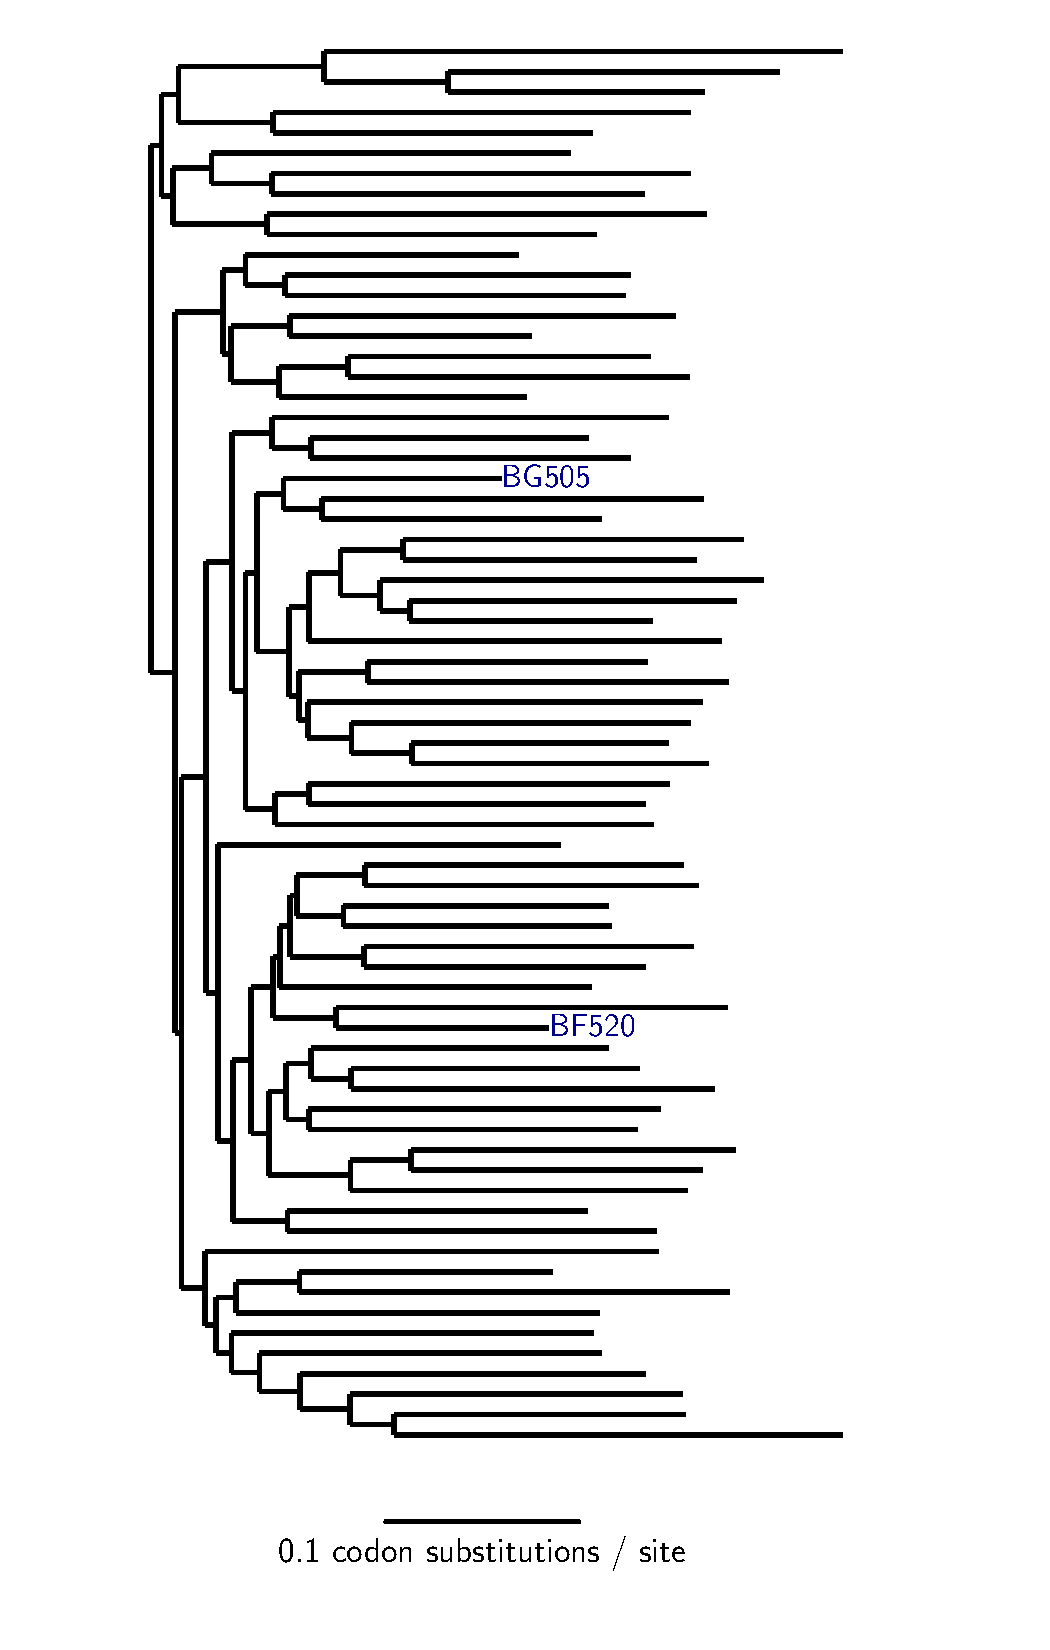
\includegraphics[clip=true, trim= 0in 0in 1in 0in, angle=-90, width=0.85\textwidth]{figures/tree_plot.pdf}}
\caption{\label{fig:tree}
Phylogenetic tree showing the relationship of BG505 and BF520 to other clade A Envs.
The tree shows the 69 Envs in the alignment in Figure~\ref{fig:tree}-source~data~\ref{figdata:alignment}, which is a subsample of clade A sequences from the group M alignment in the Los Alamos HIV sequence database (\url{http://www.hiv.lanl.gov}).
Sites not mutagenized in our experiments (the signal peptide and cytoplasmic tail) or that are poorly alignable (mostly sites in the variable loops) were masked as indicated in Figure~\ref{fig:tree}-source~data~\ref{figdata:mask}, leaving 616 alignable sites.
The pairwise identity of BG505 and BF520 to the other sequences at these alignable sites is shown in Figure~\ref{fig:tree}-Figure~supplement~\ref{figsupp:identity}.
The tree topology was inferred using \texttt{RAxML}~\citep{stamatakis2014raxml} under the GTRCAT model of nucleotide substitution, and branch lengths were optimized under the M0 version of the Goldman-Yang model~\citep{yang2000codon} using \texttt{phydms}~\citep{hilton2017phydms}.
}
\figsupp[\label{figsupp:identity}  Pairwise identity of all Env sequences in our clade A alignment to BG505 and BF520 after masking poorly alignable or non-mutagenized sites.]
{The histograms show the pairwise amino-acid identity of each Env to all other sequences in the clade A alignment in Figure~\ref{fig:tree}-source~data~\ref{figdata:alignment} after masking the sites delineated in Figure~\ref{fig:tree}-source~data~\ref{figdata:mask}.
There are 616 non-masked sites.
The pairwise protein identity between BG505 and BF520 is 86.2\% (721 of 836 sites identical) when considering \emph{all} sites, and 89.1\% (549 of 616 sites identical) when considering just the non-masked sites.}
{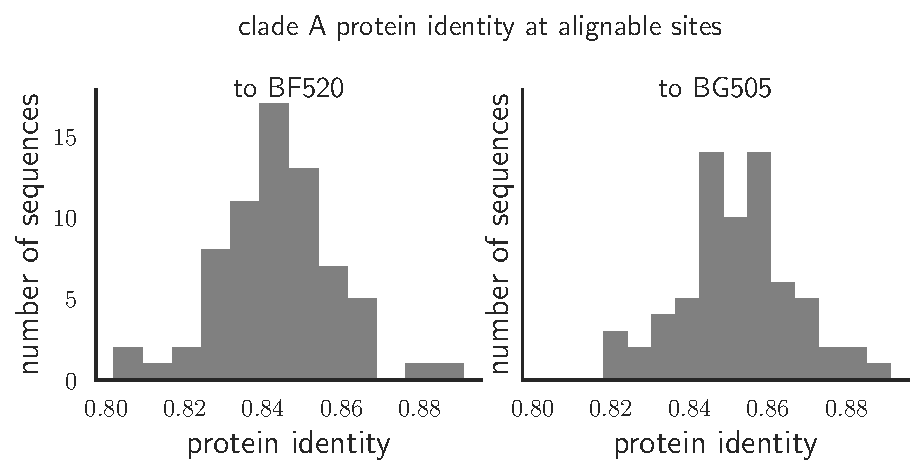
\includegraphics[width=0.7\textwidth]{figures/masked_alignment_identity.pdf}}
\figdata{\label{figdata:alignment} The alignment of clade A \textit{env} coding sequences is in \texttt{cladeA\_alignment.fasta}.}
\figdata{\label{figdata:mask} The 240 Env sites masked in all phylogenetic analyses because they were not mutagenized in our experiments or are poorly alignable are listed in \texttt{alignment\_mask.csv}.}
\end{figure}

We therefore selected Envs from two transmitted-founder viruses, BG505.W6M.C2.T332N and BF520.W14M.C2 (hereafter referred to as BG505 and BF520), that were isolated from HIV-infected infants shortly after mother-to-child transmission~\citep{goo2014early}.
The BG505 Env has been extensively studied from a structural standpoint~\citep{julien2013crystal,lyumkis2013cryo,pancera2014structure,huang2014broad,sanders2015hiv,stewart2016trimeric}, and variants of this Env are being tested as a vaccine immunogens~\citep{sanders2013next,sanders2015hiv,de2015immunogenicity}.
We used the T332N variant of BG505 Env because it has a common glycosylation site that is targeted by many anti-HIV antibodies~\citep{sanders2013next}.
The BF520 Env was isolated from an infant who developed an early broad anti-HIV antibody response~\citep{goo2014early,simonich2016hiv}.
We have previously created comprehensive codon-mutant libraries of the BF520 Env and used them to map HIV antibody escape~\citep{dingens2017comprehensive}, but these BF520 libraries have not been characterized with respect to how mutations affect viral replication.

Both BG505 and BF520 are from clade A of the major (M) group of HIV-1.
Figure~\ref{fig:tree} shows the phylogenetic relationship among these two Envs and other clade A sequences.
BG505 and BF520 have typical divergence for two clade A Envs: they are identical at 721 of the 836 pairwise-alignable protein sites (86.2\% identity), and 549 of the 616 sites (89.1\% identity) in the ectodomain and transmembrane domain that are alignable across clade A (Figure~\ref{fig:tree}-source~data~\ref{figdata:alignment}, Figure~\ref{fig:tree}-source~data~\ref{figdata:mask}).
The divergence between BG505 and BF520 therefore offers ample opportunity to investigate mutational shifts during Env evolution.

\subsection{Deep mutational scanning to measure the effects of all amino-acid mutations to each Env on HIV replication}
We have previously described a deep mutational scanning strategy for measuring how all amino-acid mutations to Env affect HIV replication in cell culture, and applied this strategy to the LAI strain~\citep{haddox2016experimental}.
In addition to using a late-stage lab-adapted HIV strain, that study had another shortcoming: the measurements were quite noisy.
Specifically, the Pearson correlation coefficients between measurements of mutational effects from independent biological replicates were in the range of $R = 0.45$ to $0.50$~\citep{haddox2016experimental}.
This noise is a problem when trying to identify differences in mutational effects between Envs, since it is only possible to reliably detect differences that exceed the magnitude of the experimental noise. 

\begin{figure}
\centerline{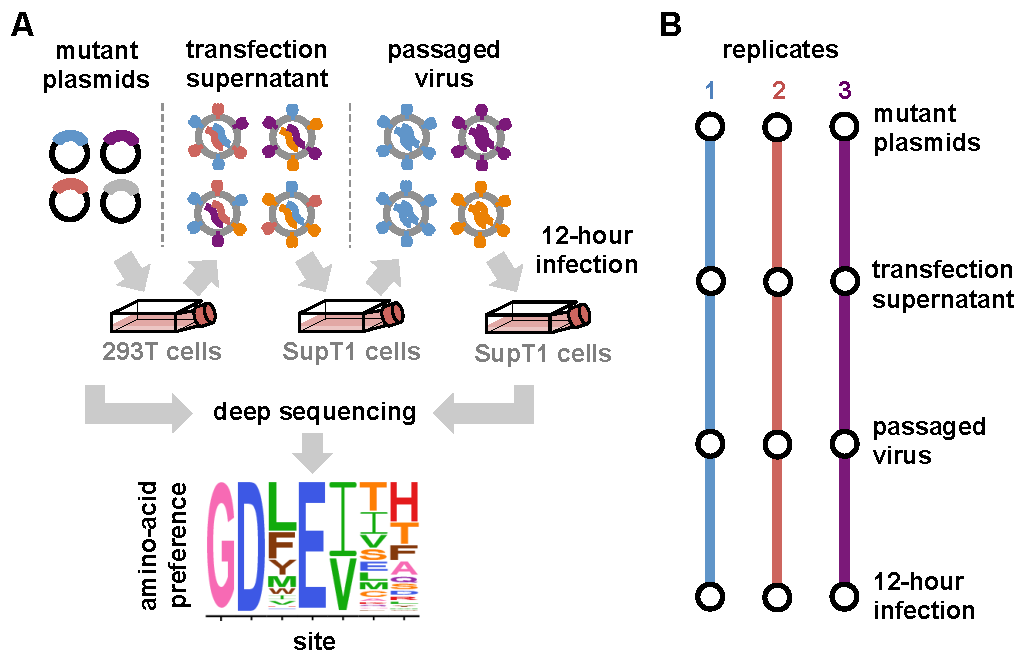
\includegraphics[width=0.75\textwidth]{figures/dms_schematic/dms_schematic.pdf}}
\caption{\label{fig:dms_schematic}
Deep mutational scanning workflow.
{\bf (A)} We made libraries of proviral HIV plasmids with random codon-level mutations in the \textit{env} gene.
The number of mutations per gene followed a roughly Poisson distribution with a mean between 1 and 1.5 (Figure~\ref{fig:dms_schematic}-Figure~supplement~\ref{figsupp:sanger}).
We transfected the plasmids into 293T cells to generate mutant viruses, which lack a genotype-phenotype link since cells are multiply transfected.
To establish a genotype-phenotype link and select for Env variants that support HIV replication, we passaged the libraries in SupT1.CCR5 cells for four days at a low multiplicity of infection (MOI) of 0.01.
To isolate the \textit{env} genes from only viruses that encoded a functional Env protein, we infected the passaged libraries into SupT1.CCR5 cells at high MOI and harvested reverse-transcribed non-integrated viral DNA after 12 hours.
We then deep sequenced the \textit{env} genes from these final samples as well as the initial plasmid library, using molecular barcoding to reduce sequencing errors.
We also deep sequenced identically handled wildtype controls to estimate error rates.
Using these sequencing data, we estimated the preference for each of the 20 amino acids at each site in Env.
These data are represented in logo plots, with the height of each letter proportional to that site's preference for that amino acid.
{\bf (B)} We conducted this experiment in full biological triplicate for both BG505 and BF520, beginning each replicate with independent creation of the plasmid mutant library.
These replicates therefore account for \emph{all} sources of noise and error in the experiments.
}
\figsupp[Sanger sequencing of selected clones from the mutant plasmid libraries.\label{figsupp:sanger}]{
We Sanger sequenced 44 clones of BG505 Env sampled roughly evenly from each of the three replicate mutant plasmid libraries.
{\bf(A)} There was an average of 1.5 mutant codons per clone, with the number of mutations per clone roughly following a Poisson distribution. 
{\bf(B)} The mutant codons had a mix of single-, double-, and triple-nucleotide changes, with an elevated number of single-nucleotide changes than expected.
{\bf(C)} Nucleotide frequencies were fairly uniform in the mutant codons.
{\bf(D)} Mutations were distributed roughly evenly along the mutagenized region of {\it env} (30-699 in the sequential numbering scheme used in this plot).
{\bf(E)} For clones with multiple mutations, we computed the pairwise distance in primary sequence between each codon mutation and plotted the cumulative distribution of these distances (red line). 
We also simulated the expected distribution of pairwise distances if mutations occurred entirely independently (blue line). 
The observed distribution is close to the expected distribution.
Comparable data for the BF520 libraries is provided in \citet{dingens2017comprehensive}.
}{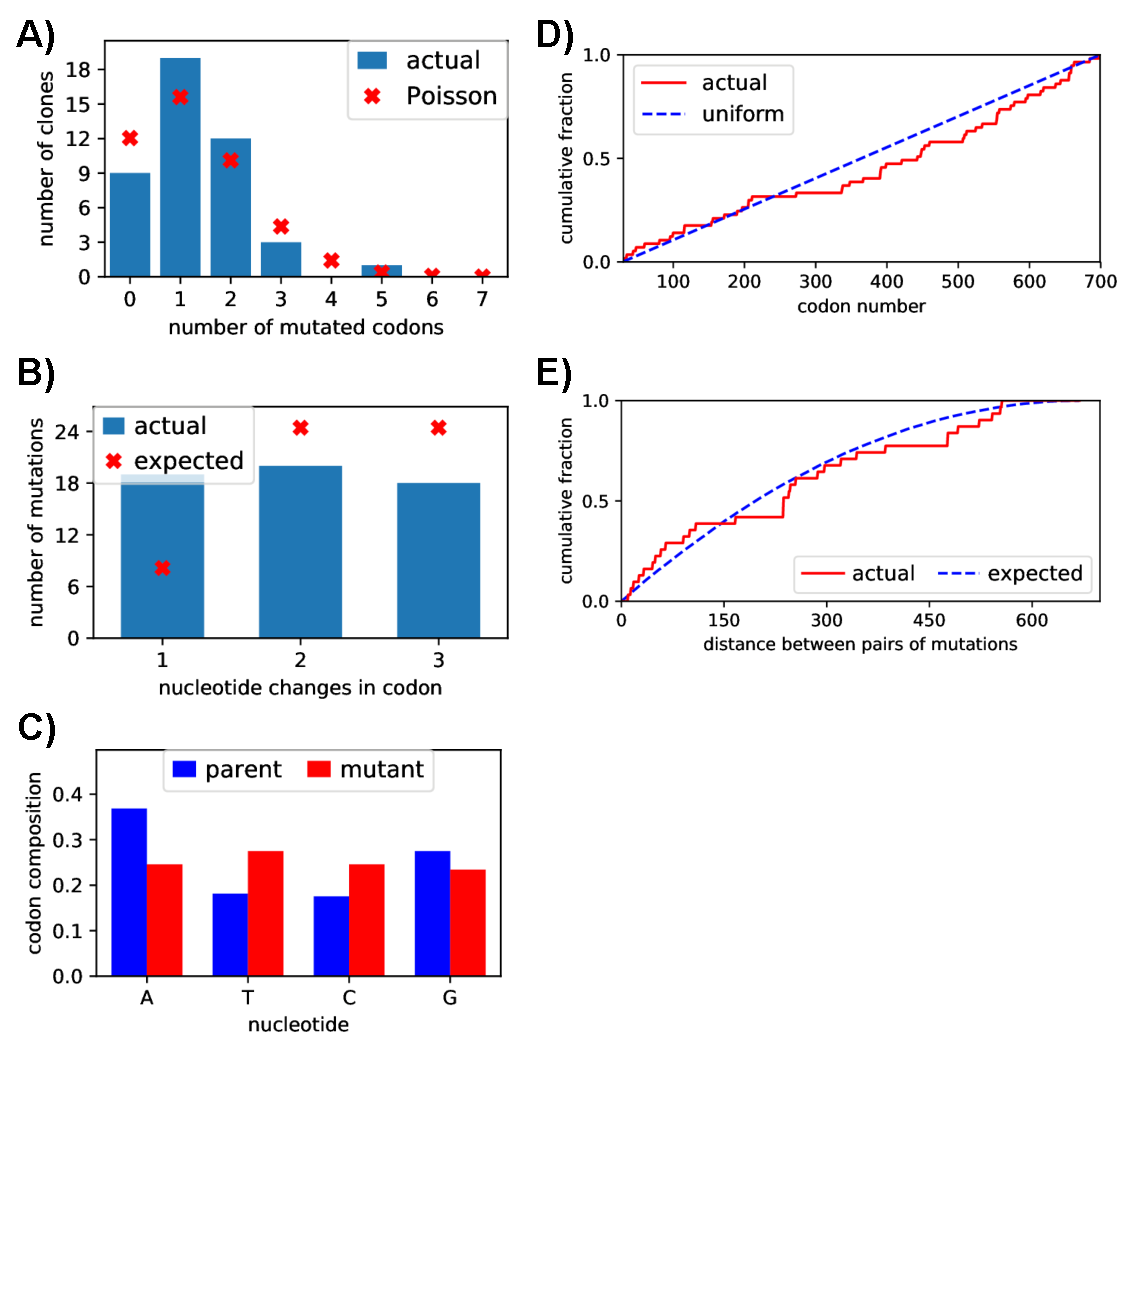
\includegraphics[width=\textwidth]{figures/sanger_sequencing_supp/sanger_sequencing_supp.pdf}}
\end{figure}

We therefore modified the deep mutational scanning strategy of \citet{haddox2016experimental} to yield the approach in Figure~\ref{fig:dms_schematic}A.
This approach had the following substantive changes: we used SupT1 cells expressing CCR5 to support replication of viruses with transmitted-founder Envs, we used more virions for the first passage ($\ge 3 \times 10^6$ versus $5\times 10^5$ infectious units per library) to avoid bottlenecking library diversity, and rather than performing a full second passage we just did a short high-MOI infection to enable recovery of \textit{env} genes from infectious virions without bottlenecking (Figure~\ref{fig:dms_schematic}A).
We performed this deep mutational scanning in full biological triplicate for both BG505 and BF520 (Figure~\ref{fig:dms_schematic}B).
Our deep mutational scanning libraries encompassed all codon mutations to all sites in Env except for the signal peptide and cytoplasmic tail.

\begin{figure}
\begin{minipage}[t]{0.34\textwidth}
{\bf \Large A} \\ 
\centerline{{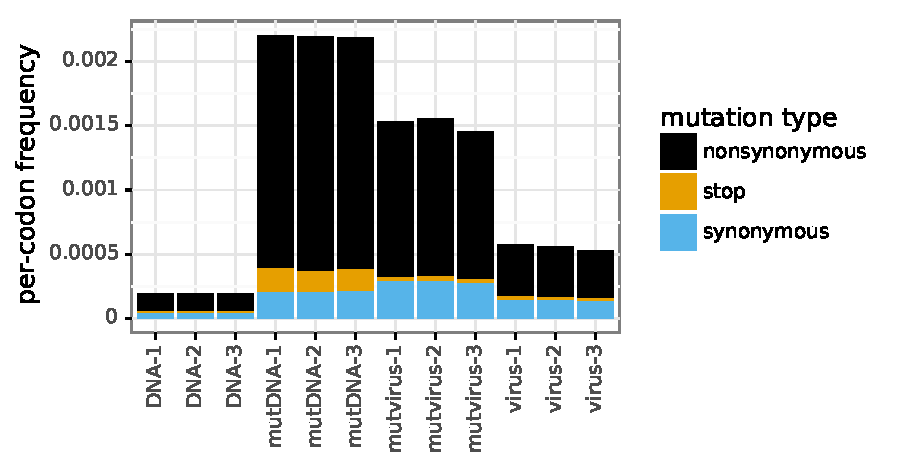
\includegraphics[clip=true, trim=4.3in 1.4in 0in 0.48in, width=0.4\textwidth]{figures/BG505_avgmutfreqs.pdf}}} 
\centerline{\small BG505}
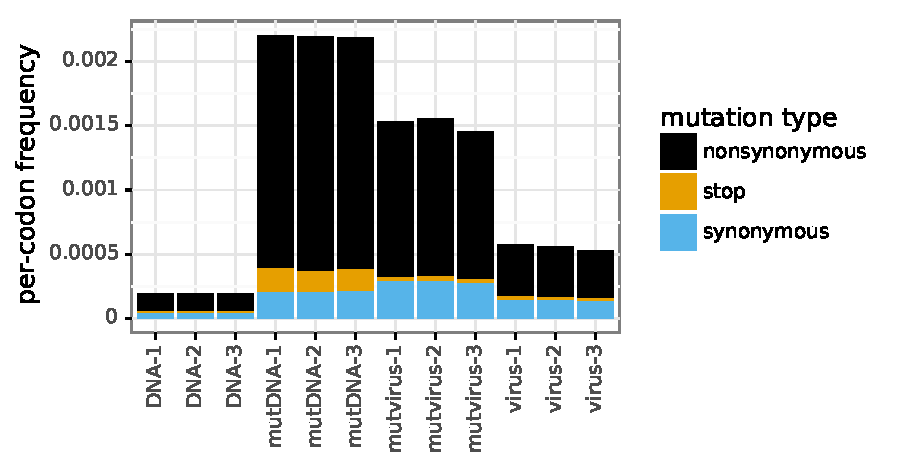
\includegraphics[clip=true, trim=0in 0in 1.7in 0in, width=\textwidth]{figures/BG505_avgmutfreqs.pdf}
\centerline{\small BF520}
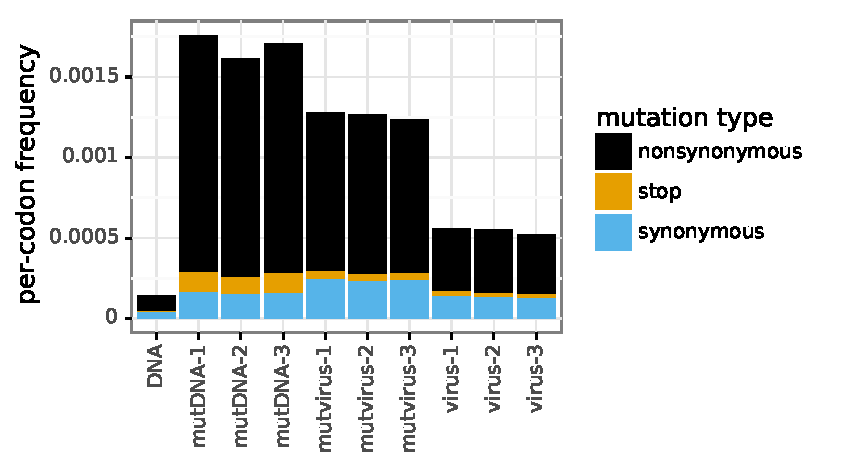
\includegraphics[clip=true, trim=0in 0in 1.7in 0in, width=0.89\textwidth]{figures/BF520_avgmutfreqs.pdf}
\end{minipage}
\begin{minipage}[t]{0.01\textwidth}
\end{minipage}
\begin{minipage}[t]{0.65\textwidth}
{\bf \Large B} \\
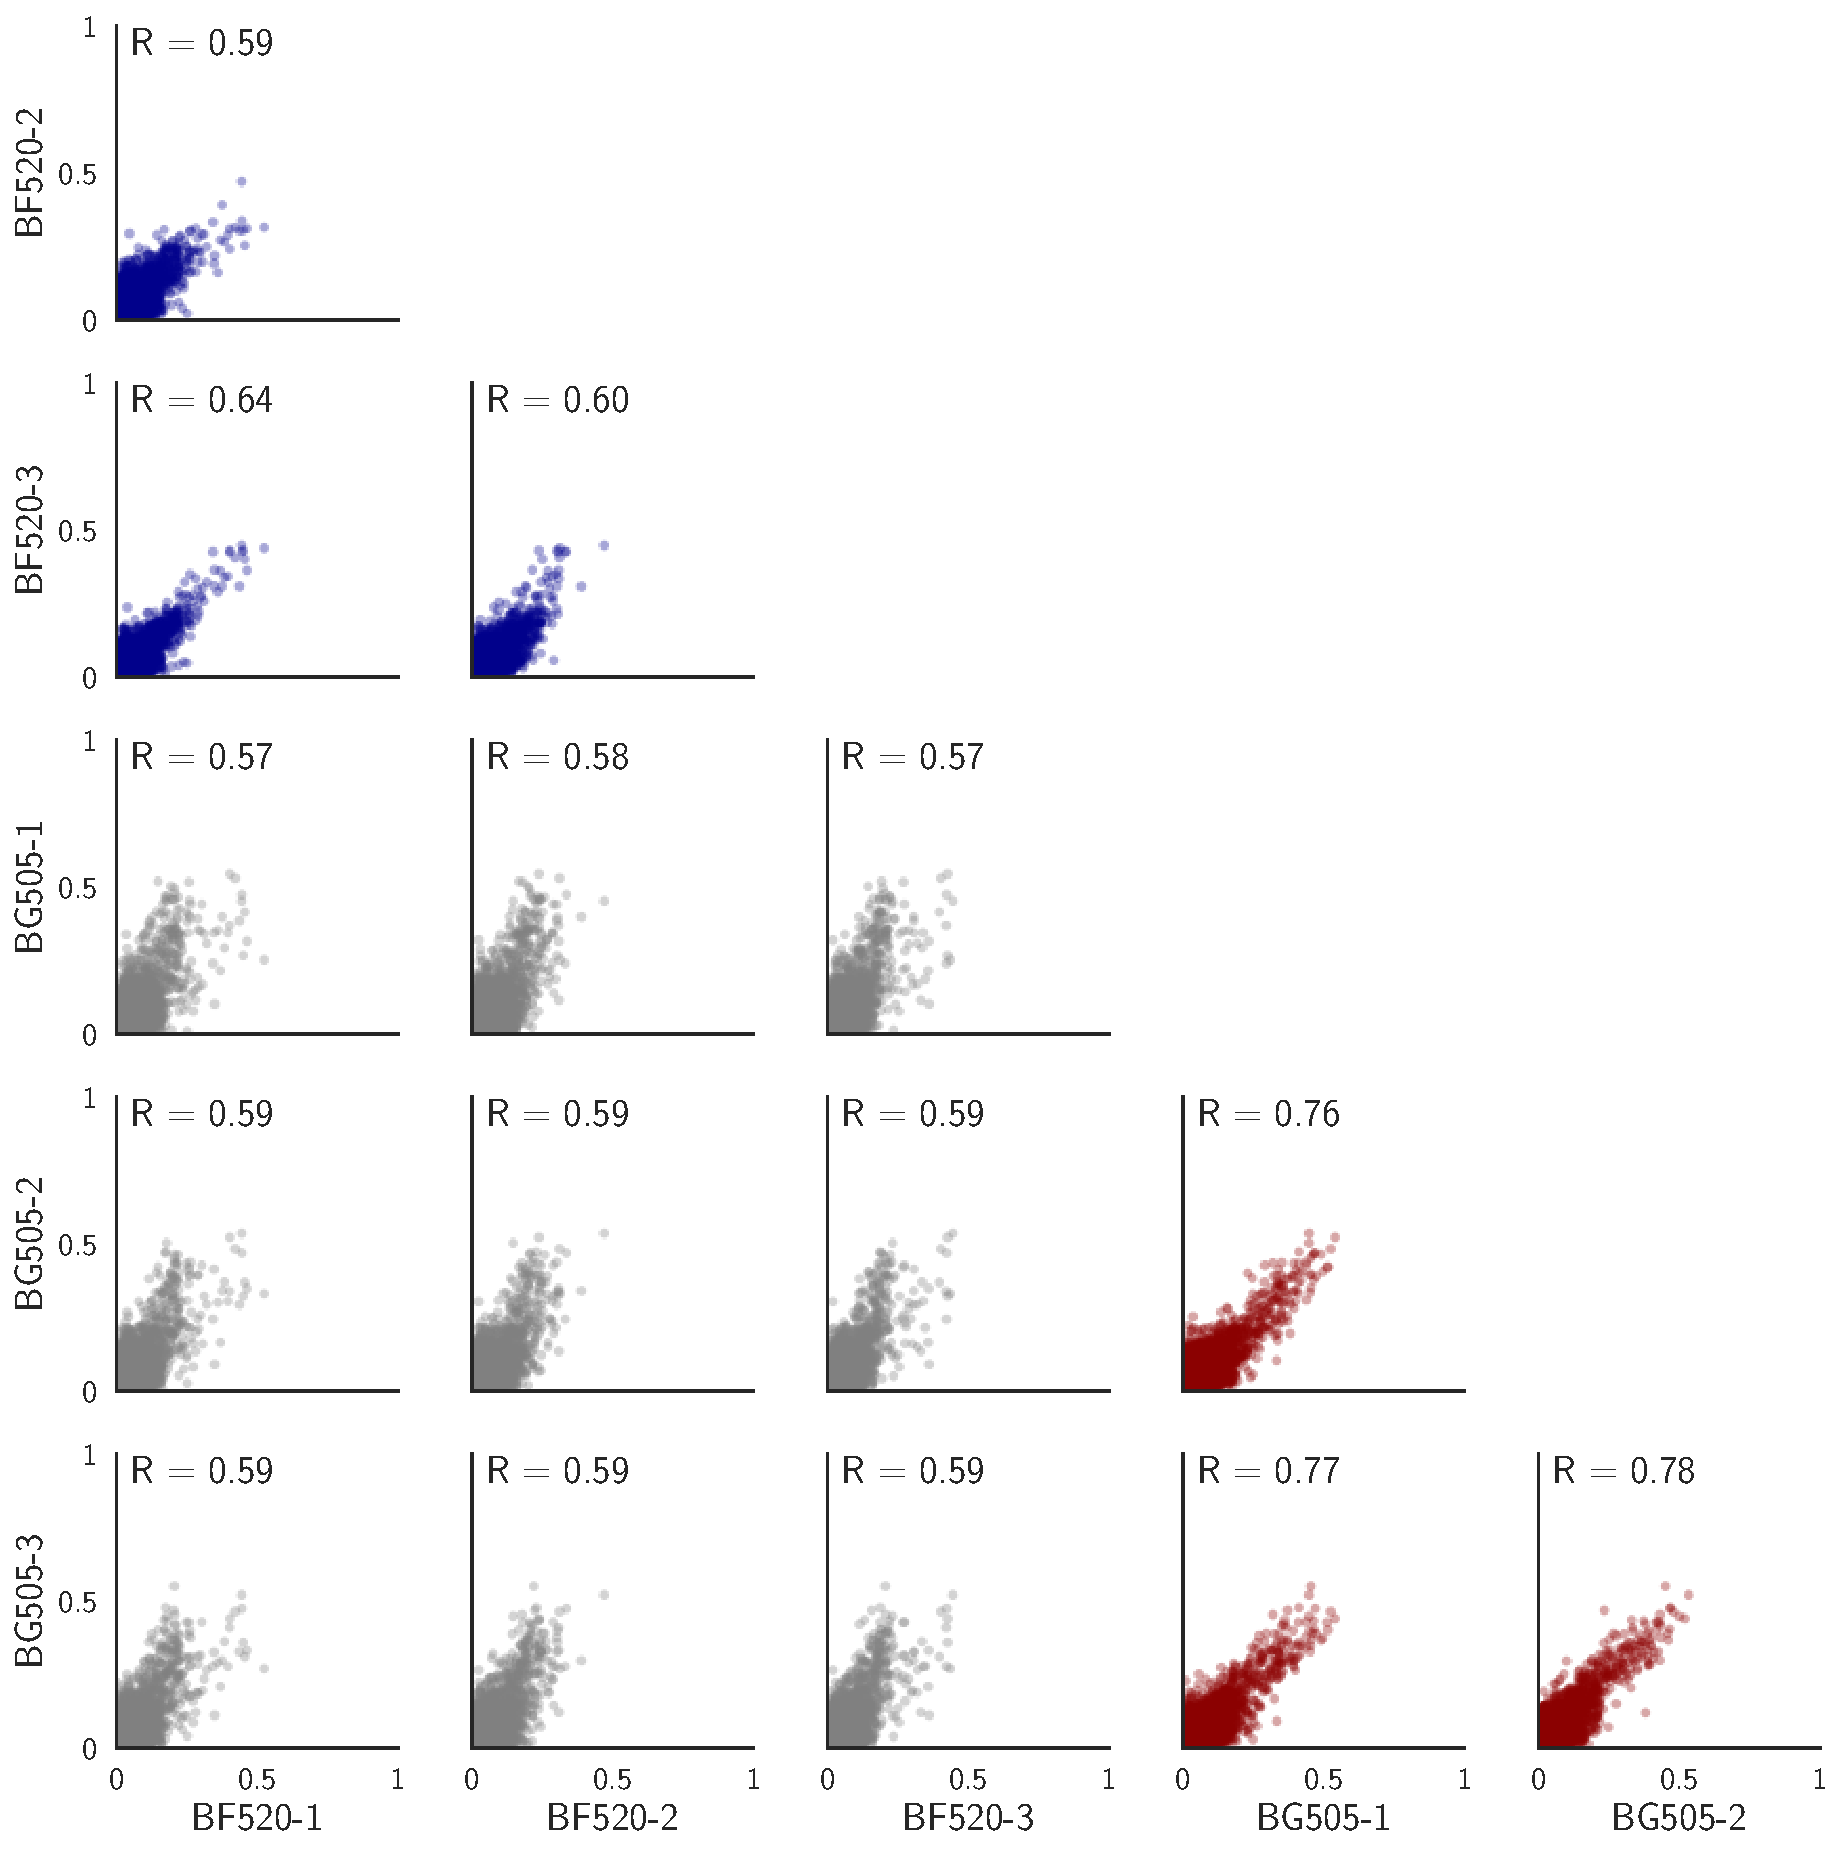
\includegraphics[width=\textwidth]{figures/allprefscorr.pdf}
\end{minipage}
\caption{\label{fig:mutfreqs}
The deep mutational scanning selects for functional Envs and yields measurements that are well correlated among replicates.
{\bf (A)}
The average per-codon mutation frequency when sequencing plasmids encoding wildtype Env (\emph{DNA}), plasmid mutant libraries (\emph{mutDNA}), mutant viruses after the final infection (\emph{mutvirus}), and virus generated from wildtype plasmids (\emph{virus}).
Mutations are categorized as nonsynonymous, synonymous, or stop codon. 
The \emph{DNA} samples show that sequencing errors are rare, and the \emph{virus} samples show that viral replication and reverse-transcription errors are well below the frequency of mutations in the \emph{mutDNA} samples.
Comparing the \emph{mutvirus} to \emph{mutDNA} shows clear purifying selection against stop codons and some nonsynonymous mutations, particularly after subtracting the background error rates given by the \emph{virus} and \emph{DNA} samples (Figure~\ref{fig:mutfreqs}-Figure~supplement~\ref{figsupp:mutfreqs}).
More extensive plots from the analysis of the deep sequencing data are in Supplementary~files~\ref{suppfile:code} and \ref{suppfile:html}.
{\bf (B)}
Correlations between replicates in the measured preferences of each site in Env for all 20 amino acids.
Blue indicates replicate measurements on BF520, red indicates replicate measurements on BG505, and gray indicates across-Env measurements of BF520 versus BG505.
$R$ is the Pearson correlation coefficient. 
The numerical values for the preferences are in Figure~\ref{fig:mutfreqs}-source~data~\ref{figdata:allprefs}.
}
\figsupp[\label{figsupp:mutfreqs} Numerical frequencies of mutations.]
{This table gives the average frequencies of nonsynonymous, synonymous, and stop-codon mutations as plotted in Figure~\ref{fig:mutfreqs}.
Note that there is only one \emph{DNA} sample for BF520, so that same sample is repeated three times in the sample in conjunction with each BF520 replicate.
We calculate the error-corrected \emph{pre}-selection mutation frequency as the \emph{mutDNA} frequency minus the \emph{DNA} frequency, and the error-corrected \emph{post}-selection mutation frequency as the \emph{mutvirus} frequency minus the \emph{virus} frequency.
We then use these error-corrected frequencies to calculate the \emph{percent} of mutations remaining after selection for each replicate and type of mutation.}
{{\small
\begin{tabular}{llrrrrrrr}
\toprule
        & sample &      DNA &   mutDNA &  mutvirus &    virus &     post &      pre &  percent \\
experiment & muttype &          &          &           &          &          &          &          \\
\midrule
BF520-1 & nonsyn & 9.41e-05 &  0.00147 &  0.000986 &  0.00039 & 0.000596 &  0.00138 &     43.3 \\
        & stop & 6.92e-06 & 0.000123 &  4.77e-05 & 3.05e-05 & 1.72e-05 & 0.000116 &     14.8 \\
        & syn & 4.27e-05 & 0.000166 &  0.000249 & 0.000141 & 0.000107 & 0.000124 &     86.6 \\
BF520-2 & nonsyn & 9.41e-05 &  0.00135 &  0.000986 & 0.000385 & 0.000601 &  0.00125 &       48 \\
        & stop & 6.92e-06 & 0.000107 &  4.33e-05 & 2.91e-05 & 1.42e-05 &   0.0001 &     14.2 \\
        & syn & 4.27e-05 & 0.000157 &   0.00024 & 0.000136 & 0.000103 & 0.000114 &     90.4 \\
BF520-3 & nonsyn & 9.41e-05 &  0.00142 &  0.000946 & 0.000362 & 0.000584 &  0.00133 &       44 \\
        & stop & 6.92e-06 & 0.000125 &  4.62e-05 & 2.72e-05 &  1.9e-05 & 0.000118 &     16.2 \\
        & syn & 4.27e-05 & 0.000162 &  0.000241 &  0.00013 & 0.000111 & 0.000119 &     93.4 \\
BG505-1 & nonsyn & 0.000137 &  0.00181 &    0.0012 & 0.000402 & 0.000802 &  0.00167 &       48 \\
        & stop & 1.01e-05 & 0.000188 &  3.38e-05 & 2.86e-05 & 5.21e-06 & 0.000178 &     2.92 \\
        & syn & 4.94e-05 &  0.00021 &  0.000296 & 0.000149 & 0.000147 &  0.00016 &     91.9 \\
BG505-2 & nonsyn & 0.000137 &  0.00182 &   0.00122 & 0.000392 & 0.000829 &  0.00168 &     49.2 \\
        & stop &  1.1e-05 & 0.000162 &  3.56e-05 & 2.62e-05 & 9.44e-06 & 0.000151 &     6.25 \\
        & syn & 5.04e-05 & 0.000209 &  0.000296 & 0.000146 &  0.00015 & 0.000159 &     94.5 \\
BG505-3 & nonsyn & 0.000134 &   0.0018 &   0.00114 & 0.000367 & 0.000774 &  0.00166 &     46.5 \\
        & stop & 9.55e-06 &  0.00017 &  3.04e-05 & 2.62e-05 &  4.2e-06 &  0.00016 &     2.62 \\
        & syn & 5.01e-05 & 0.000217 &   0.00028 & 0.000139 & 0.000141 & 0.000167 &     84.7 \\
\bottomrule
\end{tabular}

}}
\figdata{\label{figdata:allprefs} Preferences for each replicate and averages are in \texttt{all\_prefs\_unscaled.zip}.}
\end{figure}

The deep mutational scanning effectively selected for functional Env as evidenced by strong purifying selection against stop codons.
Figure~\ref{fig:mutfreqs}A shows the average frequency of mutations across Env in the plasmid mutant libraries, the mutant viruses, and wildtype controls as determined from the deep sequencing.
The mutant viruses show clear selection against stop codons and many nonsynonymous mutations (Figure~\ref{fig:mutfreqs}A).
This selection is more apparent if we correct for the background error rates estimated from the wildtype controls (Figure~\ref{fig:mutfreqs}-Figure-supplement~\ref{figsupp:mutfreqs}).
The error-corrected frequencies of stop codons drop to 3\%--16\% of their original values (Figure~\ref{fig:mutfreqs}-Figure-supplement~\ref{figsupp:mutfreqs}), with the residual stop codons probably due to some non-functional virions surviving due to complementation by other co-infecting virions. 
The error-corrected frequencies of nonsynonymous mutations also drop substantially (43\%--49\% of their original values), whereas the frequencies of synonymous mutations drop only slightly (85\%--95\% of their original values).
These trends are consistent with the fact that nonsynonymous mutations are often deleterious, whereas synonymous mutations often~\citep[although certainly not always, see][]{zanini2013quantifying} have only mild effects on viral replication.
Of course, Figure~\ref{fig:mutfreqs}A only summarizes one aspect of the deep mutational scanning data.
Supplementary~files~\ref{suppfile:code} and \ref{suppfile:html} contain detailed plots showing all aspects of the data (read depth, per-site mutation rate, etc) as generated by the \texttt{dms\_tools2} software~\citep[\url{https://jbloomlab.github.io/dms_tools2/}]{bloom2015software}.

We used the deep mutational scanning data to estimate the preference of each site in Env for each amino acid via the analysis method described in \citet{bloom2015software}.
As graphically illustrated in Figure~\ref{fig:dms_schematic}A, the preferences for each site are normalized to sum to one.
Our libraries were mutagenized at 670 sites in BG505 and 662 sites in BF520, so $670 \times 20 = 13,400$ and $662 \times 20 = 13,240$ preferences were estimated for each Env, respectively.
The correlations between the preferences from different experimental replicates are in Figure~\ref{fig:mutfreqs}B.
These replicate-to-replicate correlations are substantially higher than those for the deep mutational scanning of LAI Env by \citet{haddox2016experimental}, indicating that the experimental modifications used here were beneficial.
Because of the clear superiority of the current measurements, in this paper we do not attempt to compare to our earlier inferior LAI dataset. 
Figure~\ref{fig:mutfreqs}B also shows that while replicates are well correlated across BG505 and BF520, the replicates for BG505 are more correlated with each other than with replicates for BF520, and vice versa.
This fact hints that there are some shifts in amino-acid preferences between the two Envs -- something that is investigated with more statistical rigor later in this paper.

\subsection{Amino-acid preferences of the Envs and their relationship to HIV evolution in nature}
The most immediate question is how authentically the experimental measurements describe the actual selection on Env function in nature.
Direct comparisons between experimentally measured amino-acid preferences and amino-acid frequencies in natural sequences are confounded by the fact that the natural sequences are evolutionarily related.
This problem can be overcome by making the comparison in a phylogenetic context.
Specifically, we used our deep mutational scanning data to construct experimentally informed codon models (ExpCM's) for Env evolution~\citep{hilton2017phydms}.
Importantly, since we expect many sites in Env to be under diversifying selection from immunity, we extended the ExpCM's to draw the relative dN/dS parameter ($\omega$) from a gamma distribution as is commonly done for codon-substitution models~\citep{yang2000codon}.

\begin{table}
\begin{fullwidth}
{\centering \begin{tabular}{lrrrrrrrrr}
\toprule
           Model &  $\Delta$AIC &  LogLikelihood &  nParams &  stringency &  $\overline{\omega}$ &  $\omega_{\alpha}$ &  $\omega_{\beta}$ &  nsites $\omega_r > 1$ &  nsites $\omega_r < 1$ \\
\midrule
     ExpCM BF520 &          0.0 &       -35218.8 &        7 &         2.8 &                  1.4 &                1.0 &               0.7 &                     66 &                     35 \\
     ExpCM BG505 &        269.0 &       -35353.3 &        7 &         2.1 &                  1.3 &                0.9 &               0.7 &                     65 &                     53 \\
 Goldman-Yang M5 &       3455.1 &       -36941.4 &       12 &         nan &                  0.8 &                0.6 &               0.7 &                     14 &                    211 \\
\bottomrule
\end{tabular}
}
\caption{\label{tab:phydms}
Evolutionary models informed by the deep mutational scanning describe HIV's evolution in nature much better than a standard substitution model.
Shown are the results of maximum likelihood fitting of substitution models to the clade A phylogeny in Figure~\ref{fig:tree}.
Experimentally informed codon models~\citep[ExpCM,][]{hilton2017phydms} utilizing the across-replicate average of the deep mutational scanning describe Env's natural evolution far better than a standard codon substitution model~\citep[the M5 model of][]{yang2000codon} as judged by comparing the Akaike information criteria~\citep[$\Delta$AIC,][]{posada2004model}.
Both ExpCM models have a stringency parameter $>$1.
All models draw $\omega$ from a gamma distribution, and the table shows the mean ($\overline{\omega}$) and shape parameters ($\omega_{\alpha}$ and $\omega_{\beta}$) of this distribution.
The last two columns show the number of sites evolving faster ($\omega_r > 1$) or slower ($\omega_r < 1$) than expected at a false discovery rate of 0.05, as determined using the approach in \citet{bloom2017identification}.
Analyses were performed using \texttt{phydms} (\url{http://jbloomlab.github.io/phydms/}).
Table~\ref{tab:phydms}-source-data~\ref{tabledata:phydms} shows the results for additional substitution models.
}
\tabledata{\label{tabledata:phydms}Results for phylogenetic models where $\omega$ is not drawn from a gamma-distribution or where the preferences are averaged across sites to eliminate the site specificity are in \texttt{modelcomparison.md}.}
\end{fullwidth}
\end{table}

Table~\ref{tab:phydms} shows that phylogenetic models informed by the deep mutational scanning of either BG505 or BF520 describe the natural evolution of Env vastly better than a standard codon substitution model.
In addition to simply comparing model fits, we can interpret the model parameters.
ExpCM's have a stringency parameter that relates selection in the experiments to that in nature.
A stringency parameter $>$1 indicates that natural selection prefers the same amino acids as the experiments, but with greater stringency~\citep{hilton2017phydms}.
Both ExpCM's have stringency parameters $>$1 (Table~\ref{tab:phydms}) -- a finding that makes sense, since the stop-codon analysis in the previous section suggests that the experimental selections are more lax than natural selection on HIV.
We can also interpret the $\omega$ parameter.
For standard codon substitution models, $\omega$ is the rate of fixation of nonsynonymous mutations relative to synonymous one -- and the gene-wide average $\omega$ is almost always $<$1, since purifying selection purges many functionally deleterious amino-acid mutations even for adaptively evolving proteins~\citep{murrell2015gene}.
Indeed, Table~\ref{tab:phydms} shows that Env's gene-wide average $\omega$ is $<$1 for a standard model.
But for ExpCM, $\omega$ is the relative rate of nonsynonymous to synonymous substitutions \emph{after} accounting for functional constraints measured in the deep mutational scanning~\citep{bloom2017identification}.
Table~\ref{tab:phydms} shows that the ExpCM's have a gene-wide average $\omega$ that is $>$1, indicating that immune selection drives Env to fix amino-acid mutations faster than expected under a null model that only accounts for functional constraints.

\begin{figure}
\begin{fullwidth}
{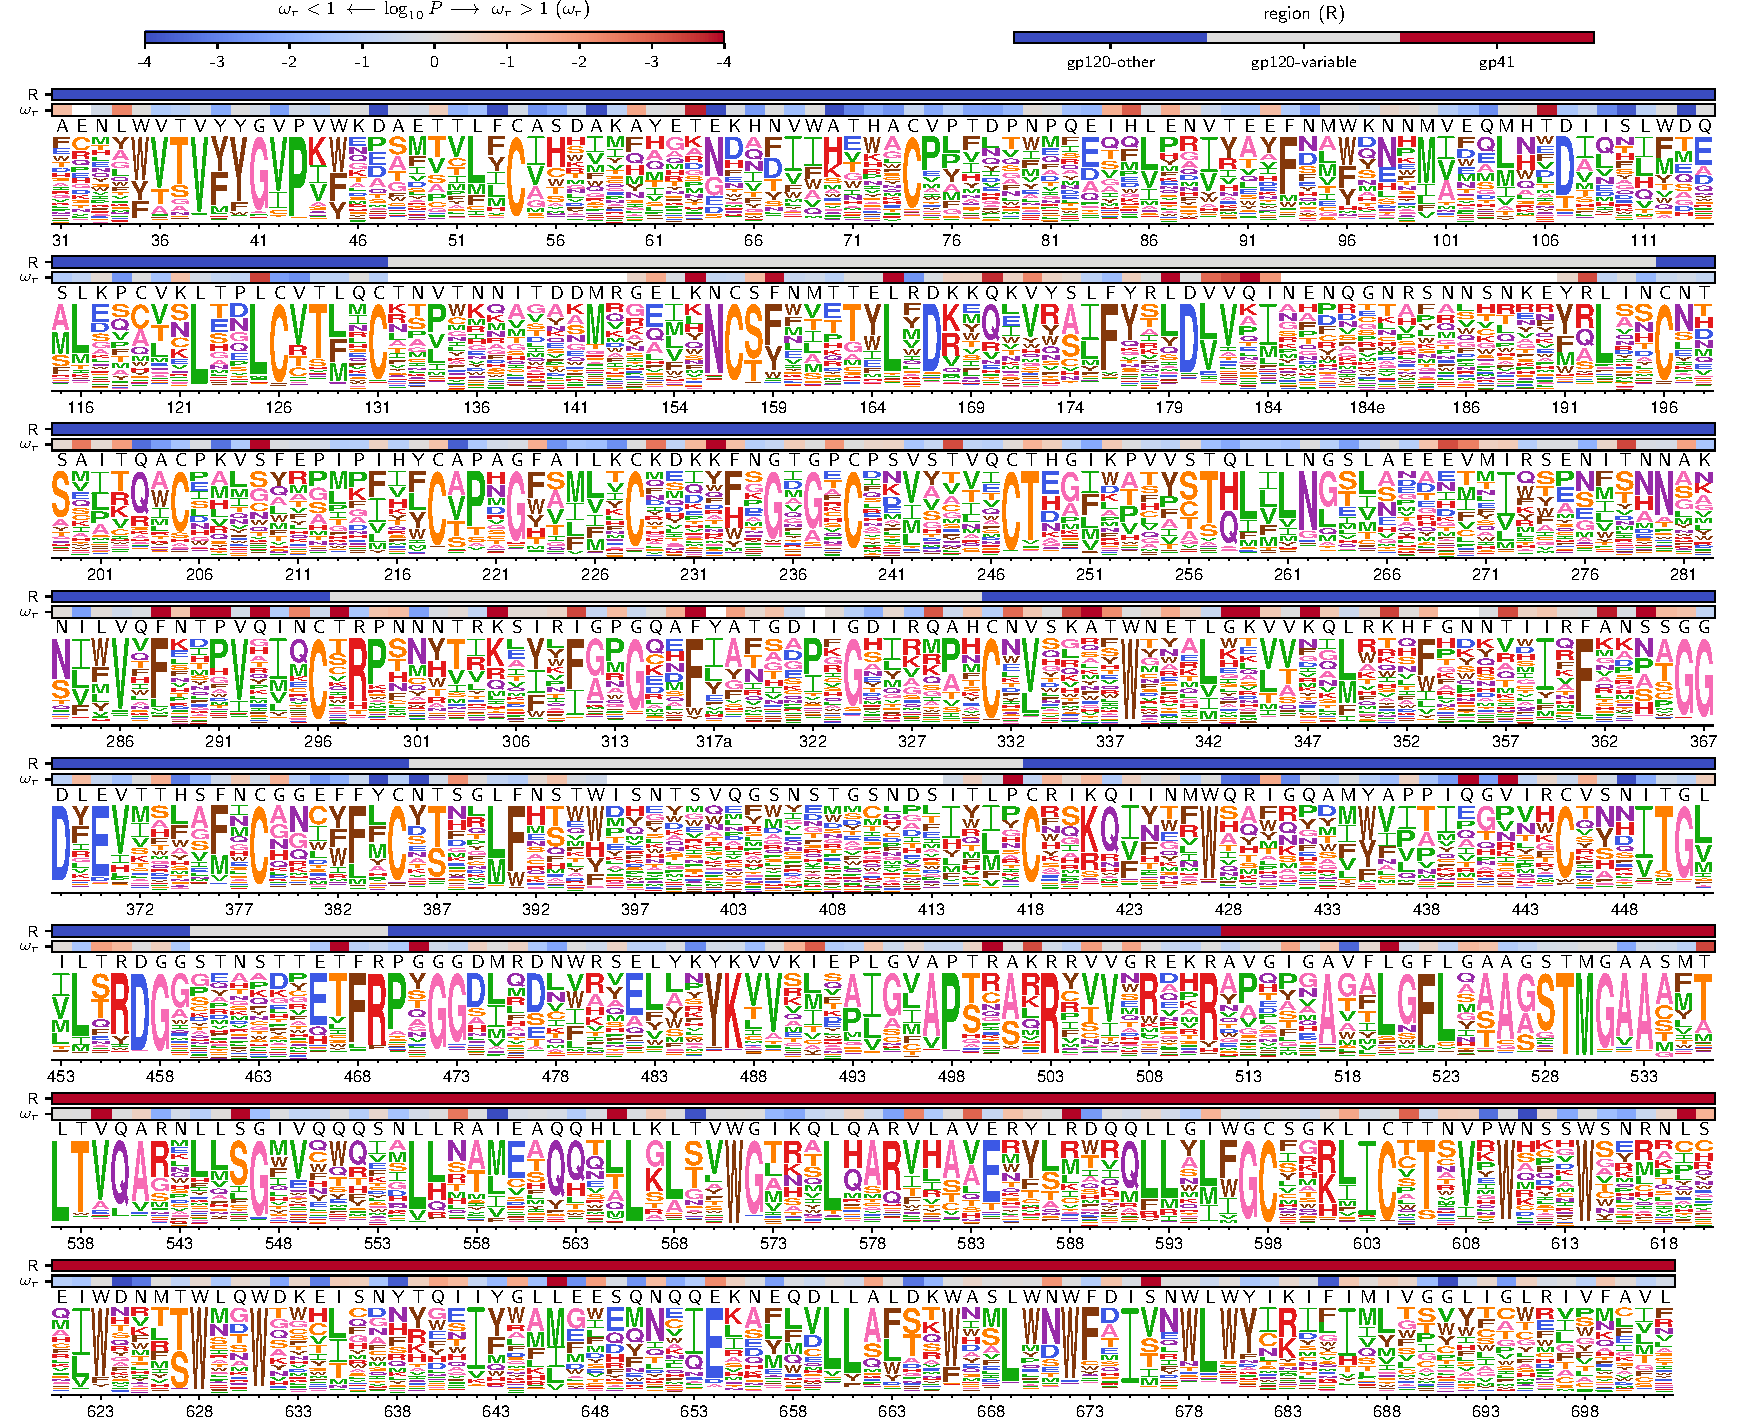
\includegraphics[width=1.3\textwidth]{figures/BG505_prefs.pdf}}
\caption{\label{fig:BG505prefs}
Amino-acid preferences for the BG505 Env.
At each site, the height of the letter is proportional for that site's preference for that amino acid.
The top color bar indicates the region of Env (gp120 variable loop, gp120 not variable loop, or gp41).
The lower color bar indicates the evidence that the site evolves faster ($\omega_r > 1$) or slower ($\omega_r < 1$) than expected given the experiments~\citep[see][]{bloom2017identification}.
The letters above the logos indicate the wildtype amino acid in BG505.
Sites are numbered using the HXB2 scheme~\citep{korber1998numbering}).
This logo plot shows the site-specific amino-acid preferences for BG505 after averaging the replicates and re-scaling by the stringency parameter in Table \ref{tab:phydms}.
The figure was generated using \texttt{dms\_tools2}~\citep[\url{https://jbloomlab.github.io/dms_tools2/}]{bloom2015software}, which in turn utilizes \texttt{weblogo}~\citep{crooks2004weblogo}.
}
\figdata{The numerical values of the amino-acid preferences plotted in this figure are in \texttt{rescaled\_BG505\_prefs.csv.}}
\figdata{The sequence of BG505 Env and mapping from sequential (\emph{original} column) to HXB2 numbering (\emph{new} column) is in \texttt{BG505\_to\_HXB2.csv}.}
\figdata{The $\omega_r$ values and associated $P$-values for BG505 in HXB2 numbering are in \texttt{BG505\_omegabysite.tsv}.}
\end{fullwidth}
\end{figure}

\begin{figure}
\begin{fullwidth}
{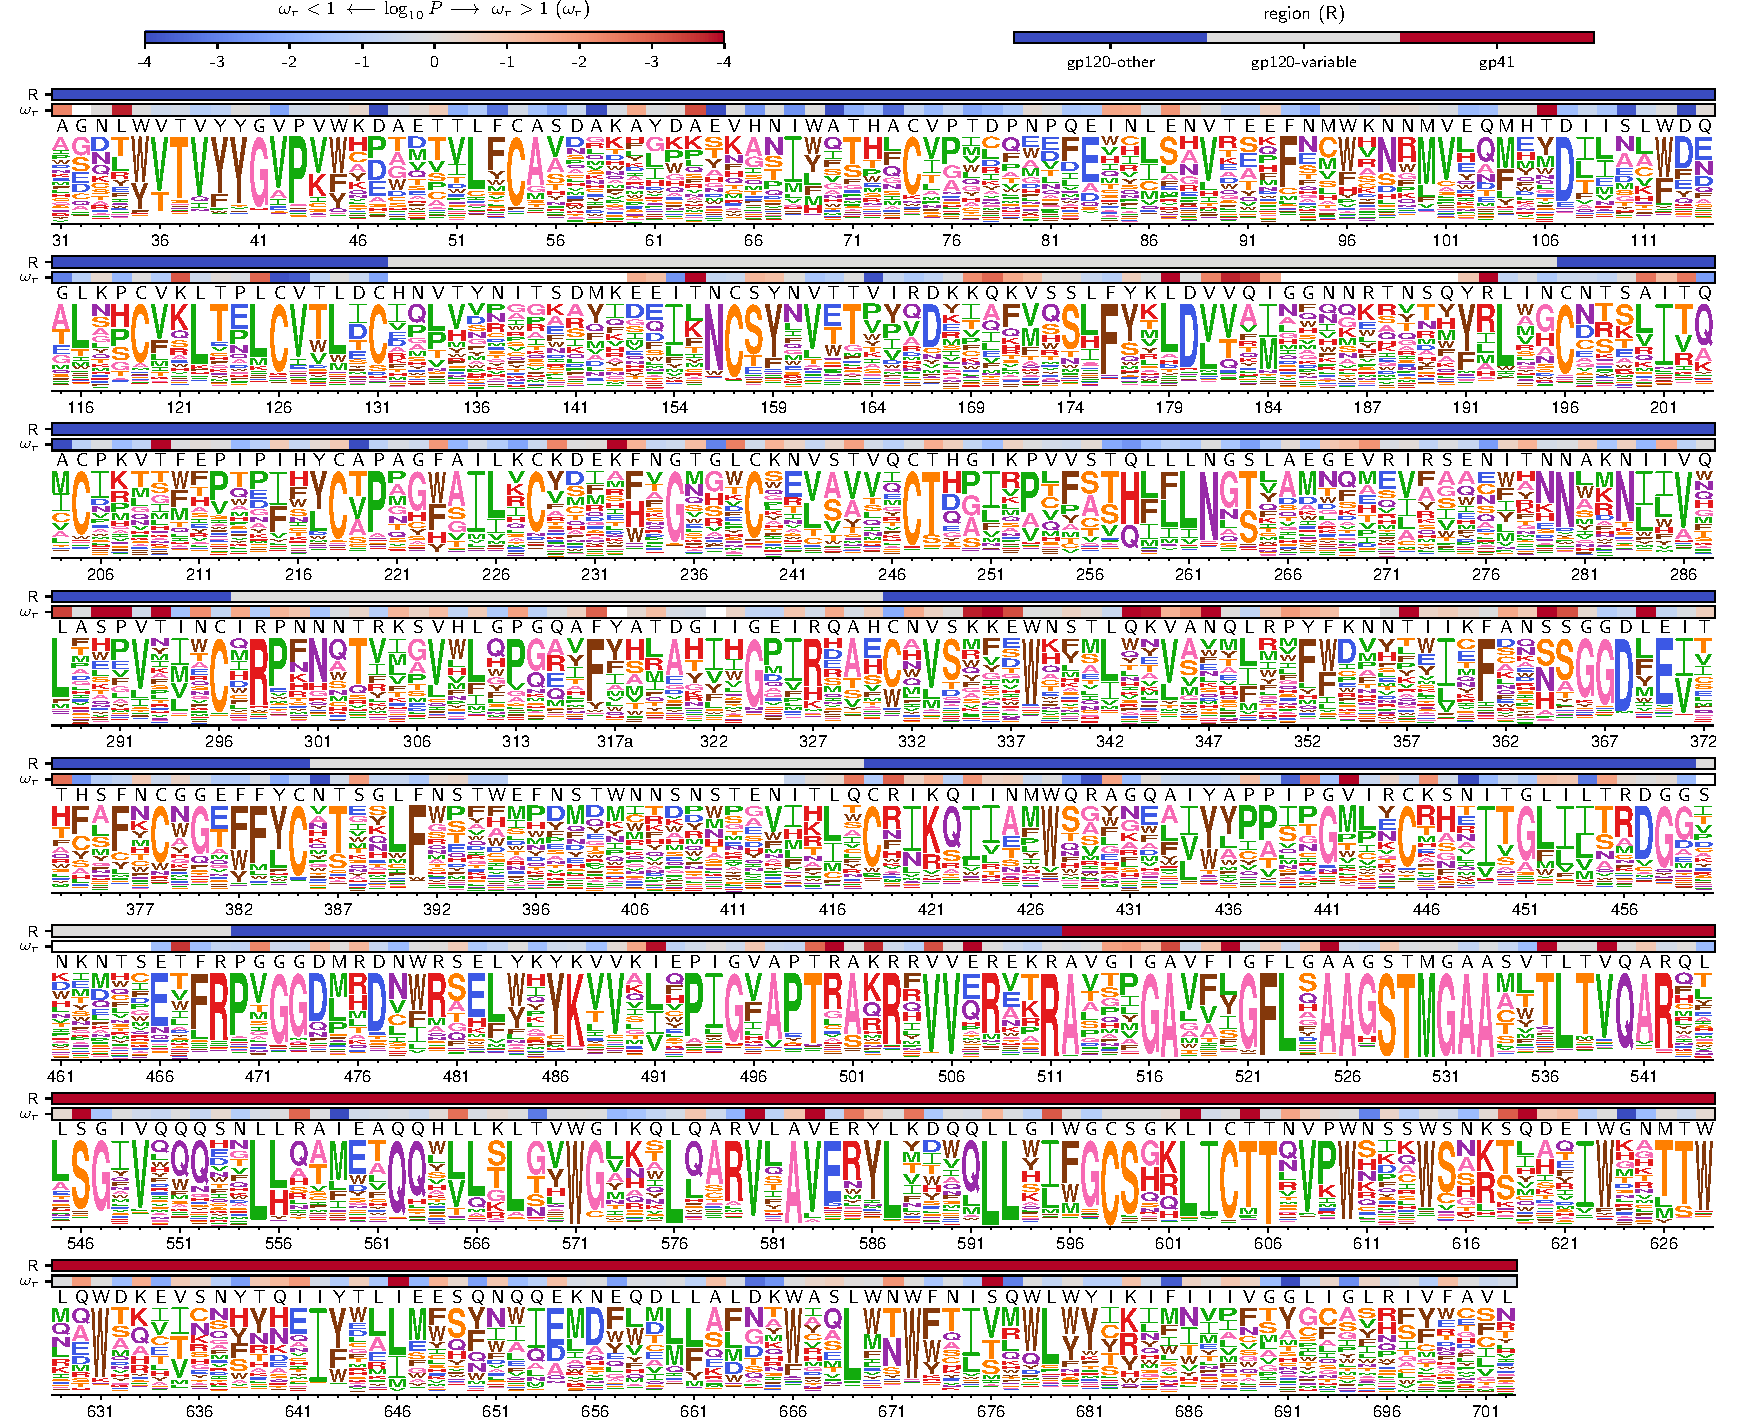
\includegraphics[width=1.3\textwidth]{figures/BF520_prefs.pdf}}
\caption{\label{fig:BF520prefs}
Amino-acid preferences for the BF520 Env.
This figure is the same as Figure~\ref{fig:BG505prefs} except that it shows the data for BF520 instead of BG505.
}
\figdata{The numerical values of the amino-acid preferences plotted in this figure are in \texttt{rescaled\_BF520\_prefs.csv.}}
\figdata{The sequence of BF520 Env and mapping from sequential (\emph{original} column) to HXB2 numbering (\emph{new} column) is in \texttt{BF520\_to\_HXB2.csv}.}
\figdata{The $\omega_r$ values and associated $P$-values for BF520 in HXB2 numbering are in \texttt{BG505\_omegabysite.tsv}.}
\end{fullwidth}
\end{figure}

A more qualitative way to assess if the deep mutational scanning authentically describes selection on Env function is to visually compare the measurements with existing knowledge.
Figures~\ref{fig:BG505prefs} and \ref{fig:BF520prefs} show the across-replicate average of the amino-acid preferences for each Env after re-scaling by the stringency parameters in Table~\ref{tab:phydms}.
At sites of known functional importance, these preferences are usually consistent with prior knowledge.
For instance, residues T257, D368, E370, W427, and D457 are important for Env binding to CD4~\citep{olshevsky1990identification}, and all these amino acids are highly preferred in our deep mutational scanning (Figures~\ref{fig:BG505prefs} and \ref{fig:BF520prefs}).
Likewise, Env has 10 disulfide bonds (linking sites 54-74, 119-205, 126-196, 131-157, 218-247, 228-239, 296-331, 378-445, 385-418, and 598-604), most of which are important for function~\citep{van2008only} -- and the cysteines at these sites are highly preferred in our deep mutational scanning.
The deep mutational scanning is also consistent with prior knowledge about sites that are tolerant of mutations.
For instance, Env has five variable loops that mostly evolve under weak constraint in nature~\citep{starcich1986identification,zolla2010structure} -- and most sites in these loops are mutationally tolerant in our deep mutational scanning (see sites indicated by gray overlay bars in Figures~\ref{fig:BG505prefs} and \ref{fig:BF520prefs}, such as 132 to 195).
It is beyond the scope of this paper to catalog associations between our measurements and all other prior mutational studies of Env, but we anticipate that the complete maps of mutational effects in Figures~\ref{fig:BG505prefs} and \ref{fig:BF520prefs} will be useful for future sequence-structure-function studies.

\subsection{Shifts in amino-acid preferences between BG505 and BF520}
The most fundamental question that we seek to address is how similar the effects of mutations are between the two Envs.
We can get some hint simply by examining Figure~\ref{fig:mutfreqs}B, which shows the correlations among the amino-acid preferences measured for all experimental replicates for both BG505 and BF520.
All replicates are strongly correlated with each other regardless of which Env was used, indicating that many aspects of the preferences are conserved between BG505 and BF520.
But the correlations between replicate measurements for the same Env are always greater than or equal to those for replicate measurements on different Envs, suggesting at least some shifts in preferences between BG505 and BF520.
However, simply comparing correlation coefficients in this way does not identify specific sites where mutational effects have shifted, nor does it quantify the magnitude of any shifts.

\begin{figure}
\begin{fullwidth}
{\bf \Large A} \hspace{0.61\textwidth} {\bf \Large B} \\
\hspace{0.01\textwidth} 
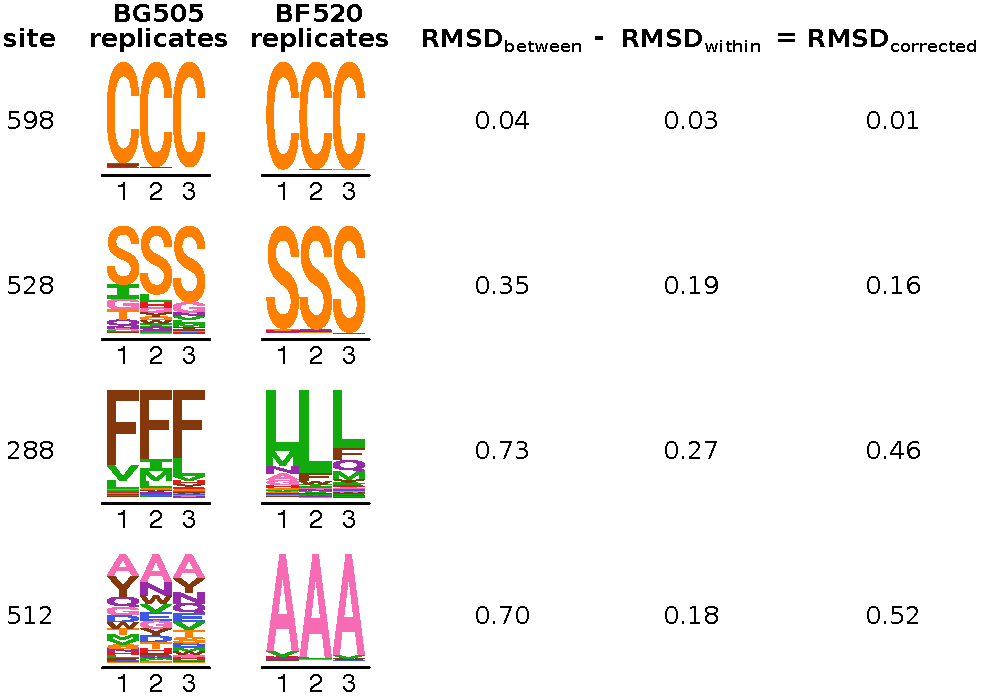
\includegraphics[width=0.58\textwidth]{figures/prefs_distance/prefs_distance.pdf}
\hspace{0.03\textwidth}
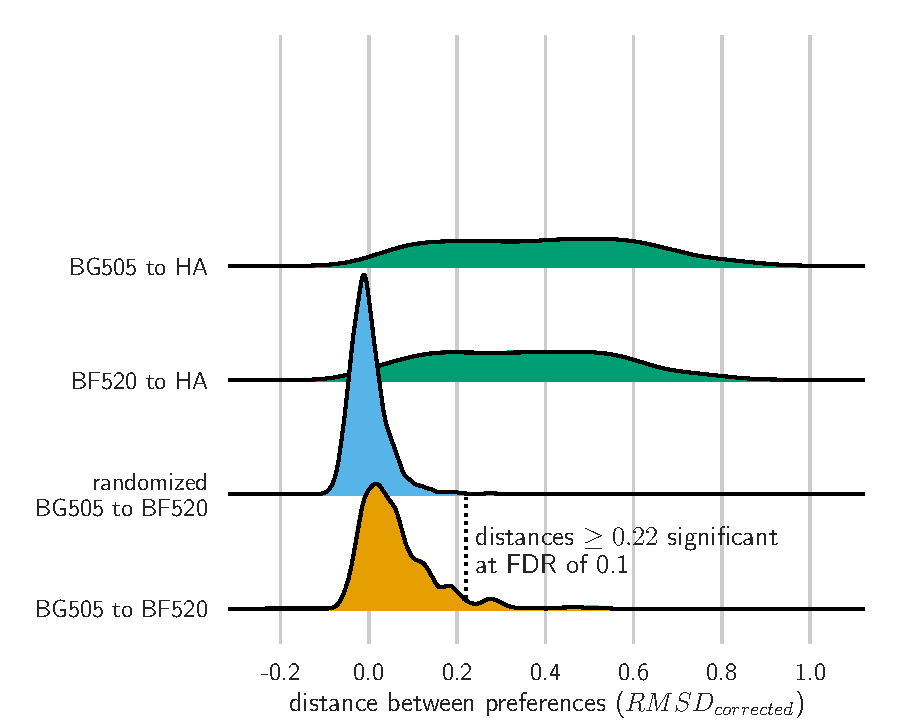
\includegraphics[clip=true, trim=0in 0in 0in 1.2in, width=0.68\textwidth]{figures/distance_distribution.pdf}
\vspace{0.15in}
\\ 
{\bf \Large C} \\
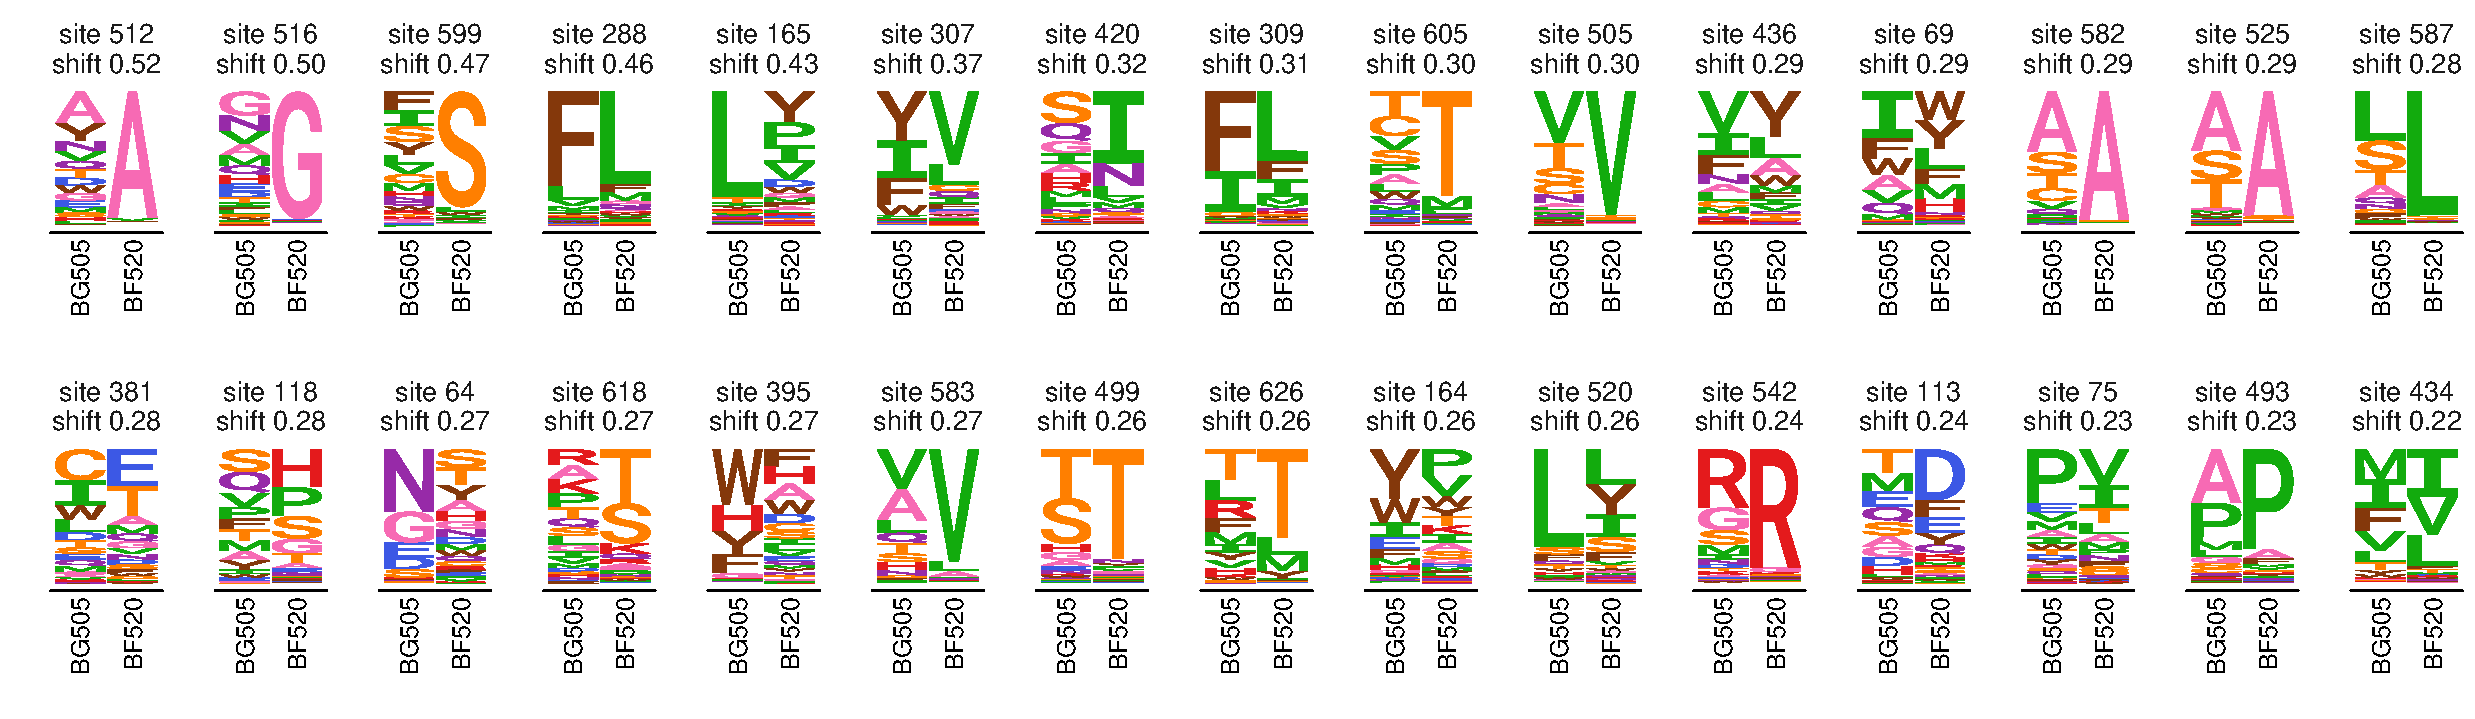
\includegraphics[width=1.3\textwidth]{figures/shifted_sites.pdf}
\caption{\label{fig:prefsdist}
Env sites with shifted amino-acid preferences between BG505 and BF520.
{\bf (A)} Calculation of the corrected distance between the amino-acid preferences of BG505 and BF520 at five example sites.
We have triplicate measurements for each Env.
We calculate the distance between each pair of replicate measurements, and group these into comparisons \emph{between} the two Envs and \emph{within} replicates for the same Env.
We compute the root-mean-square distance (RMSD) for both sets of comparisons, which we denote as RMSD$_{\rm{between}}$ and RMSD$_{\rm{within}}$.
The latter quantity is a measure of experimental noise.
The noise-corrected distance between Envs at a site, RMSD$_{\rm{corrected}}$, is simply the distance between the two Envs minus this noise.
{\bf (B)} The bottom distribution (orange) shows the corrected distances between BG505 and BF520 at all alignable sites.
The next distribution (blue) is a null generated by computing the corrected distances on all randomizations of the replicates among Envs.
The top two distributions (green) compare Env to the non-homologous influenza hemagglutinin (HA) protein~\citep{doud2016accurate} simply putting sites into correspondence based on sequence number.
We compute the $P$-value that a site has shifted between BG505 and BF520 as the fraction of the null distribution that exceeds that shift, and identify significant shifts at a false discovery rate (FDR) of 0.1 using the method of \citet{benjamini1995controlling}.
Using this approach, 30 of the 659 sites have significant shifts (corrected distance $\ge$0.22).
{\bf (C)} All sites that have significantly shifted their amino-acid preferences at an FDR of 0.01.
For each site, the logo stacks show the across-replicate average preferences for BG505 and BF520.
The sites are sorted by the magnitude of the shift.
}
\figdata{\label{figdata:prefsdist}The corrected distances between BG505 and BF520 at each site are in \texttt{BG505\_to\_BF520\_prefs\_dist.csv}.}
\end{fullwidth}
\end{figure}

We therefore used a more rigorous approach to identify sites where the amino-acid preferences differ between BG505 and BF520 by an amount that exceeds the noise in our experiments.
We first re-scaled the preferences from each experimental replicate by the stringency parameter for that Env from Table~\ref{tab:phydms} to calibrate all measurements to the stringency of natural selection.
We then identified the 659 sites in the mutagenized regions of Env that are pairwise alignable between BG505 and BF520 (Figure~\ref{fig:prefsdist}-source~data~\ref{figdata:prefsdist}).
For each site, we calculated the shift in amino-acid preferences between Envs using an approach similar to that of \citet{doud2015site} as illustrated in Figure~\ref{fig:prefsdist}A.
This approach calculates the magnitude of the shift after correcting for experimental noise by comparing the differences in preferences between replicates for BG505 and BF520 to the differences between replicates for the same Env.
Figure~\ref{fig:prefsdist}A shows this calculation for a site that has not shifted (site 598, which strongly prefers cysteine in both Envs), the most shifted site (512, which shifts from being mutationally tolerant in BG505 to strongly preferring alanine in BF520), and several other sites with more intermediate behaviors.

The overall distribution of shifts between BG505 and BF520 is shown in Figure~\ref{fig:prefsdist}B.
Most sites have relatively small shifts (close to zero), although there is a long tail of sites with large shifts.
This tail reaches its upper value with site 512, which has a shift of 0.52 out of a maximum possible of 1.0.
How should we interpret this distribution -- have mutational effects shifted a lot, or not very much?
We can establish an upper-bound for how much sites might shift by comparing Env to a \emph{non}-homologous protein.
Figure~\ref{fig:prefsdist}B shows the distribution of shifts when comparing Env to influenza's hemagglutinin protein, which has previously had its amino-acid preferences measured by deep mutational scanning~\citep{doud2016accurate} .
Most sites have large shifts between Env and hemagglutinin, with the typical shift being $\sim$0.4 and some approaching the maximum value of 1.0.
We can also establish a lower-bound by creating a null distribution for the expected shifts if all differences are simply due to experimental noise.
This null distribution is created by randomizing the experimental replicates among Envs.
Figure~\ref{fig:prefsdist}B shows that the null distribution is more peaked at zero than the real distribution, and does not have the same prominent tail of sites with large shifts.
The answer to the question of how much mutational effects have shifted is therefore nuanced: they have substantially shifted at some sites, but remain vastly more similar between the two Envs than between two unrelated proteins. 

We can use the null distribution to identify sites where the shifts between BG505 and BF520 are significantly larger than the noise in our experiments (Figure~\ref{fig:prefsdist}B).
There are 30 such sites at a false discovery rate of 0.1.
Figure~\ref{fig:prefsdist}C shows the amino-acid preferences of these significantly shifted sites for each Env.
For the majority of shifted sites, one Env prefers a specific amino acid whereas the other Env tolerates many amino acids; for instance, see sites 512, 516, 165, 605 and 505 in Figure~\ref{fig:prefsdist}C.
Such broadening and narrowing of a site's mutational tolerance is often observed during protein evolution, and is frequently~\citep{wang2002evolution,bloom2006protein,gong2013stability,kumar2017stability} although not always~\citep{starr2017alternative} linked to changes in protein stability -- with a more stable protein typically being more mutationally tolerant.
Work with engineered Env protein in the form of ``SOSIP'' trimer~\citep{binley2000recombinant,sanders2002stabilization} has shown that BG505 SOSIP is more thermostable than BF520 SOSIP~\citep{verkerke2016epitope}.
The fact that the shifted sites usually (although not always, see sites 165 and 520 in Figure~\ref{fig:prefsdist}C) tolerate more mutations in the more stable BG505 Env is therefore consistent with the view that increased protein stability is often associated with shifts towards higher mutational tolerance.

However, not all of the significantly shifted sites show a simple pattern of broadening or narrowing of mutational tolerance.
For instance, site 288 does not alter its mutational tolerance but rather flips its rather narrow amino-acid preference from phenylalanine in BG505 to leucine in BF520 (Figure~\ref{fig:prefsdist}C).
Several other sites show similar but somewhat milder flips in which amino acids they prefer.
In later sections, we investigate evolutionary and structural characteristics of these shifted sites -- but as is often the case for proteins as complex as Env, we are unable to rationalize many aspects of the observed sequence-function relationships, including the cause of these shifts.
 
 An important caveat to the foregoing analysis is that it only identifies the 30 sites with shifts that exceed the experimental noise.
 It is possible that other sites have undergone small shifts not detectable by our experiments -- indeed, a recent study by \citet{starr2017pervasive} found that small shifts are common during the evolution of the Hsp90 protein in yeast.
 However, it is not technically feasible to experimentally measure the fitness effects of mutations to HIV with the same precision as for model organisms such as yeast.
Therefore, we can only conclude that 30 Env sites have undergone \emph{detectable} shifts in amino-acid preferences between BG505 and BF520.
It is possible that more sensitive experiments would find additional small shifts. 

\subsection{Structural and evolutionary properties of shifted sites}

\begin{figure}
{\bf \Large A} \\
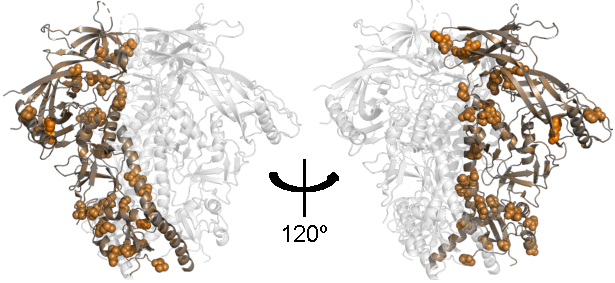
\includegraphics[width=0.8\textwidth]{figures/shifts_on_structure/shifts_on_structure.pdf}
\\
{\bf \Large B} \hspace{0.28\textwidth} {\bf \Large C} \hspace{0.28\textwidth} {\bf \Large D} \\
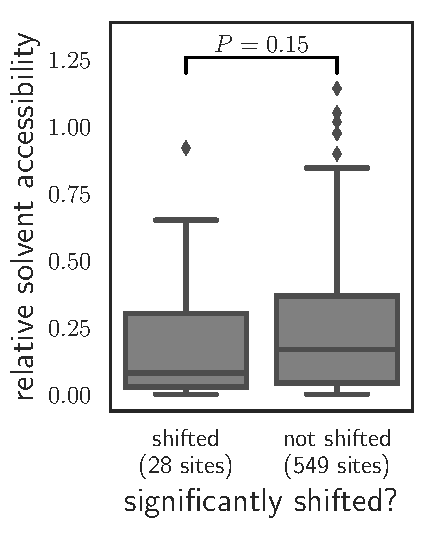
\includegraphics[width=0.28\textwidth]{figures/rsa_vs_shifts.pdf}
\hspace{0.01\textwidth}
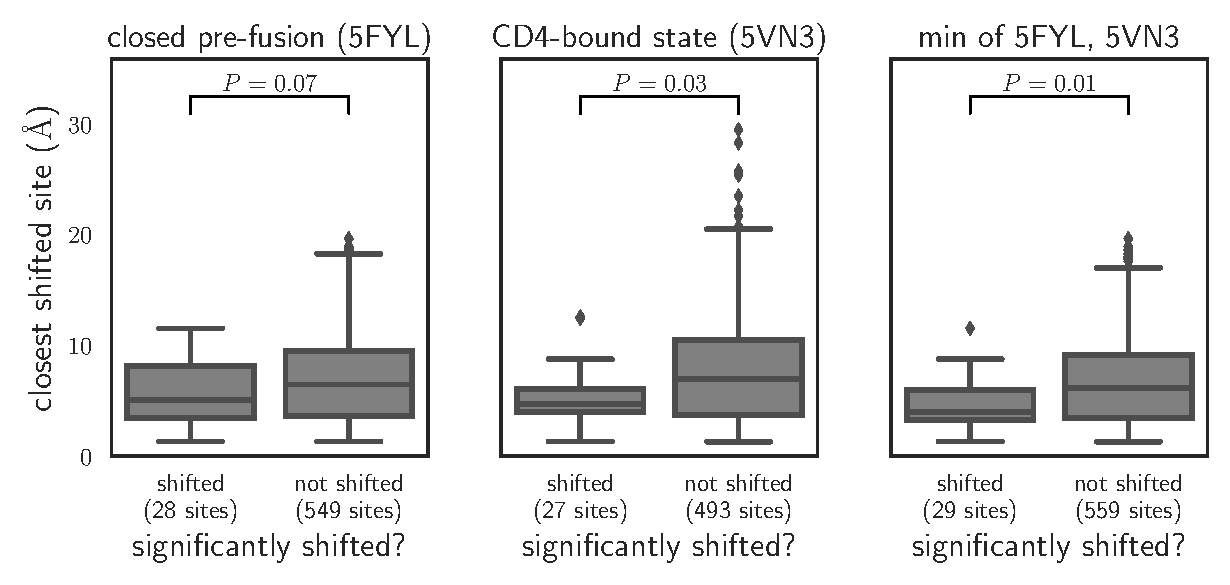
\includegraphics[width=0.28\textwidth]{figures/shifts_proximity.pdf}
\hspace{0.01\textwidth}
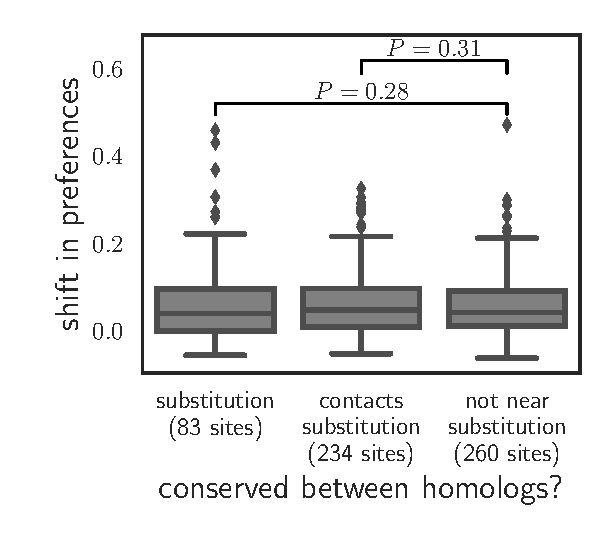
\includegraphics[width=0.4\textwidth]{figures/conservation_vs_shifts.pdf} 
\caption{\label{fig:shiftfeatures}
Characteristics of significantly shifted sites.
{\bf (A)} One monomer of the Env trimer~\citep[PDB 5FYL;][]{stewart2016trimeric} is colored from gray to orange according to the magnitude of the mutational shift at each site (orange indicates large shift).
Sites that are significantly shifted according to Figure~\ref{fig:prefsdist}B are in spheres, and all other sites are in cartoon representation.
{\bf (B)} 
There is no significant difference in relative solvent accessibility of sites that have and have not undergone significant shifts.
The absolute solvent accessibility of each site was calculated using DSSP~\citep{kabsch1983dictionary} and normalized to a relative solvent accessibility using the absolute accessibilities from \citet{tien2013maximum}.
{\bf (C)} 
Sites of significant shifts are clustered in Env's structure.
Shown is the distance of each significantly shifted and not-shifted site to the closest other shifted site.
{\bf (D)}
Large mutational shifts are \emph{not} strongly enriched at sites that have substituted between BG505 and BF520. 
The plot shows the magnitudes of the shifts among the 83 crystallographically resolved sites that have substituted between BG505 and BF520, the 234 sites that physically contact a substitution in the Env structure (any non-hydrogen atom within 3.5\angstrom), and all other sites.
Figure~\ref{fig:shiftfeatures}-Figure~supplement~\ref{figsupp:subs_shifts} shows that there is a modest borderline-significant tendency of significantly shifted sites to have substituted.
All panels only show the 577 sites that are resolved in the crystal structure.
Of the 30 significantly shifted sites in Figure~\ref{fig:prefsdist}B, only 28 are crystallographically resolved.
Structural distances and solvent accessibilities were calculated using all monomers in the trimer.
$P$ values were calculated using the Mann-Whitney $U$ test.
}
\figsupp[\label{figsupp:subs_shifts}Statistical testing of whether significantly shifted sites are more likely to have substituted between BG505 and BF520.]
{The sites of significant shifts as determined in Figure~\ref{fig:prefsdist}B are somewhat more likely to be among the sites that have substituted between BG505 and BF520.
However, this association is only borderline statistically significant, with $P = 0.055$ using a Fisher's exact test.}
{\begin{tabular}{lrr}
\toprule
substituted &  False &  True  \\
significant\_shift &        &        \\
\midrule
False             &    545 &     84 \\
True              &     22 &      8 \\
\bottomrule
\end{tabular}
}
\end{figure}

What distinguishes the sites that have undergone significant shifts?
Figure~\ref{fig:shiftfeatures}A shows the locations of the shifted sites on the crystal structure of Env.
There is no visually obvious tendency for shifted sites to preferentially be on Env's surface or in its core, and a statistical analysis (Figure~\ref{fig:shiftfeatures}B) finds no association between a site's relative solvent accessibility and whether its amino-acid preferences have shifted.
However, visual inspection of Figure~\ref{fig:shiftfeatures}A does suggest that the sites of significant shifts tend to cluster in Env's structure, and a statistical analysis confirms that this is the case (Figure~\ref{fig:shiftfeatures}C).
Therefore, the factors that drive shifts in Env's mutational tolerance often affect physically interacting clusters of residues in a coordinated fashion.

An obvious hypothesis is that strongly shifted sites have substituted between BG505 and BF520, or physically contact such substitutions.
According to this hypothesis, substitutions would alter the local physicochemical environment of the substituted site and its neighbors, thereby shifting the amino-acid preferences of sites in the physical cluster.
But surprisingly, the typical magnitude of shifts is not significantly larger at sites that have substituted or contact substitutions compared to other sites in Env (Figure~\ref{fig:shiftfeatures}C).
There is a borderline trend for the significantly shifted sites to be more likely to have substituted between BG505 and BF520 (Figure~\ref{fig:shiftfeatures}-Figure~supplement~\ref{figsupp:subs_shifts}), but most shifted sites have not substituted (only 8 of the 30 shifted sites differ in amino-acid identity between the two Envs).
The lack of strong enrichment in shifts at substituted sites contrasts with previous protein-wide experimental~\citep{doud2015site} and simulation-based~\citep{pollock2012amino,shah2015contingency} studies of shifting amino-acid preferences, which found that shifts were dramatically more pronounced at sites of substitutions.
The difference may arise because these earlier studies examined proteins that are fairly conformationally static (absolutely so in the case of the simulations).
On the other hand, Env is an extremely complex and conformationally dynamic protein~\citep{munro2014conformational,ozorowski2017open}, which may increase the opportunities for long-range epistasis to enable substitutions at one site to shift the amino-acid preferences of distant sites.

\subsection{Entrenchment of substitutions modestly contributes to mutational shifts}

\begin{figure}
\centerline{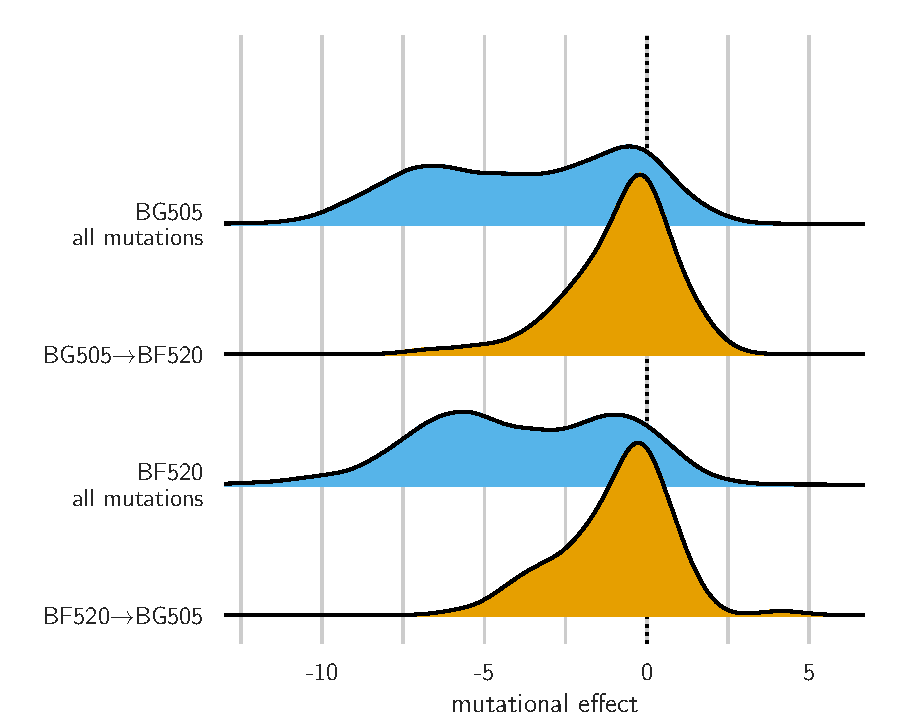
\includegraphics[clip=true, trim=0in 0in 0in 0.7in, width=0.68\textwidth]{figures/entrenchment.pdf}}
\caption{\label{fig:entrenchment}
Entrenchment of substitutions during Env evolution.
There are 12,521 possible amino-acid mutations at the 659 mutagenized sites alignable between BG505 and BF520.
The blue densities show the effects of all these mutations to each Env.
The orange densities show the effects of just the 92 mutations that convert BG505 to BF520 or vice versa.
In the absence of entrenchment, mutating a site in BG505 to its identity in BF520 should have the opposite effect of mutating the site in BF520 to its identity in BG505.
In this case, we would expect the BF520$\rightarrow$BG505 distribution to be the mirror image of the BG505$\rightarrow$BF520 distribution -- and both distributions should be centered around zero if the two Envs are equivalently functional.
Instead, mutating a site in either Env to its identity in the other Env tends to be deleterious, indicating that substitutions are often entrenched in the Env in which they have fixed.
The effect of a mutation is quantified as the ratio of the site's preference for the mutant amino acid to the preference for the wildtype amino acid.
}
\end{figure}

One idea that has recently gained support in the protein-evolution field is that substitutions become ``entrenched'' by subsequent evolution.
Specifically, after \citet{pollock2012amino} suggested that amino-acid preferences systematically shift at sites of substitutions, \citet{shah2015contingency} formalized a definition of entrenchment which \citet{starr2017pervasive} subsequently reduced to experimental practice.
Entrenchment is the tendency of a mutational reversion to become increasingly unfavorable as a sequence evolves.
Given two homologs, if there is no entrenchment then the effect of mutating a site in the first homolog to its identity in the second will simply be the opposite of mutating the site in the second homolog to its identity in the first.
But if there is entrenchment, then both mutations will be unfavorable, since the site is entrenched at its preferred identity in each homolog.

Figure~\ref{fig:entrenchment} shows the distribution of effects for mutating all sites that differ between BG505 and BF520 to the identity in the other Env.
As expected under entrenchment, the average effect of these mutations is deleterious -- although there are a substantial number of sites where the mutational flips are not deleterious. 
We can get some sense of the magnitude of the entrenchment by comparing the effects of the BG505$\leftrightarrow$BF520 mutations to the distribution of effects of all possible amino-acid mutations (Figure~\ref{fig:entrenchment}).
This comparison shows that even unfavorable inter-Env mutational flips are generally more favorable than random amino-acid mutations.
Therefore, entrenchment occurs for some but not all substitutions that distinguish BG505 and BF520, and the magnitude of entrenchment is less than the effect of a typical random mutation.
Entrenchment of substitutions therefore contributes to some of the mutational shifts.
But given that many of these shifts occur at sites that do not even differ between the Envs (Figure~\ref{fig:shiftfeatures}D), entrenchment of substitutions is clearly not the only cause of the shifting amino-acid preferences.


\subsection{Comparing selection in the lab to natural selection}
Our experiments measure the effects of mutations on viral replication in a T-cell line in the lab.
But HIV actually evolves in humans, where additional selection pressures on Env are undoubtedly present.
For instance, antibody pressure might increase the rate of evolution at some sites~\citep{albert1990rapid,wei2003antibody,richman2003rapid}, whereas pressure to mask certain epitopes~\citep{kwong2002hiv} might add constraint at other sites. 
Comparing selection in our experiments to natural selection can identify sites that are under such additional pressures during HIV's actual evolution in humans.

\begin{figure}
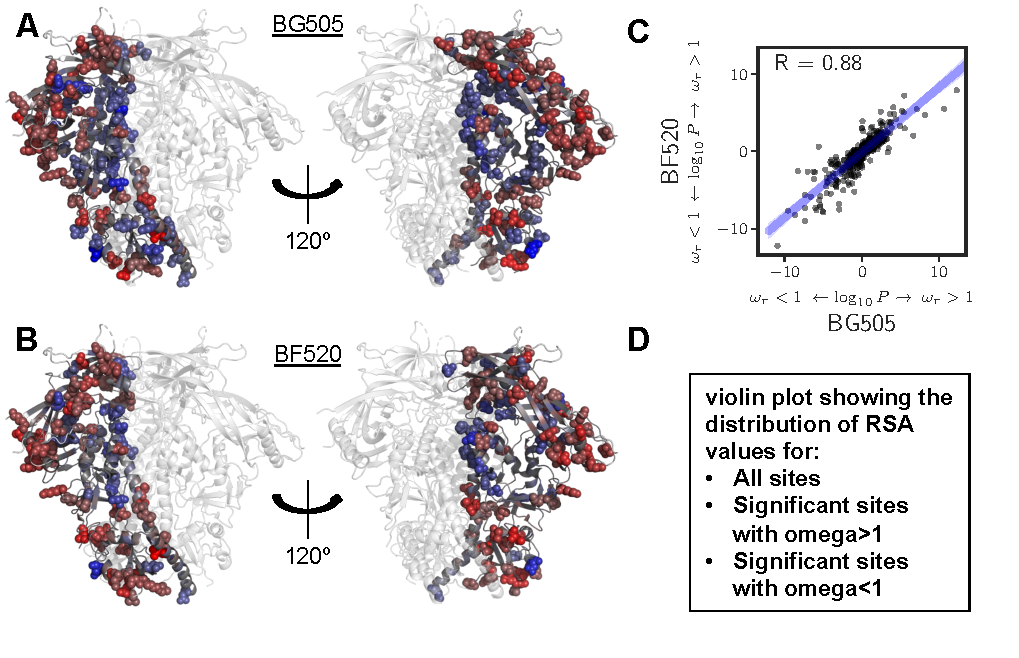
\includegraphics[width=1.0\textwidth]{figures/omegabysite_structural_analysis/omegabysite_structural_analysis.pdf}
\caption{\label{fig:divsel}
Sites in Env that evolve faster or slower in nature than expected given the functional constraints measured in the lab.
We calculated the statistical evidence ($P$ value) that each site evolves faster ($\omega_r > 1$) or slower ($\omega_r < 1$) than expected given the experimentally measured amino-acid preferences using the method of \citet{bloom2017identification}.
We then converted the $P$ values to $Q$ values to interpret them in the context of the false discovery rate~\citep{storey2003statistical}
{\bf (A)}
One monomer of the Env trimer~\citep[PDB 5FYL;][]{stewart2016trimeric} is colored from blue to red based on the strength of evidence that sites are evolving slower (blue) or faster (red) than expected given the BG505 experiments.
Sites where the rate of evolution is significantly different than expected at a false discovery rate of 0.05 are shown in spheres.
{\bf (B)}
Sites of slower or faster than expected evolution given the BF520 experiments.
For both sets of experiments, sites that evolve faster or slower than expected are often on Env's surface (Figure~\ref{fig:divsel}-Figure~supplement~\ref{figsupp:divselRSA}).
{\bf (C)}
The results are similar regardless of whether the BG505 or BF520 experiments are used.
Many of the sites of slower-than-expected evolution are asparagines in N-linked glycosylation motifs.
All sites that evolve slower than expected for both experimental datasets are in Figure~\ref{fig:divsel}-Figure~supplement~\ref{figsupp:slower}.
{\bf (D)} 
A large cluster of sites that evolve slower than expected is likely involved in Env's transition between open and closed conformational states.
Gray boxes indicate sites that \citet[PDB 5VN3]{ozorowski2017open} proposed form the hydrophobic network that regulates the conformational change; blue boxes and sticks indicate sites that evolve slower than expected.
All analyses used the phylogenetic tree in Figure~\ref{fig:tree}.
}
\figsupp[\label{figsupp:divselRSA}Relative solvent accessibilities of sites evolving faster or slower than expected.]{
Sites are grouped by whether they have $\omega_r > 1$ (diversifying selection) or $\omega_r < 1$ (purifying selection) at $Q < 0.05$ in \emph{both} homologs, or whether they do fall into neither of these categories.
Relative solvent accessibilities were calculated as in Figure~\ref{fig:shiftfeatures}.
As can be seen from these box plots with overlaid points for each site, sites of both diversifying and purifying selection tend to have higher relative solvent accessibility than other sites.
}{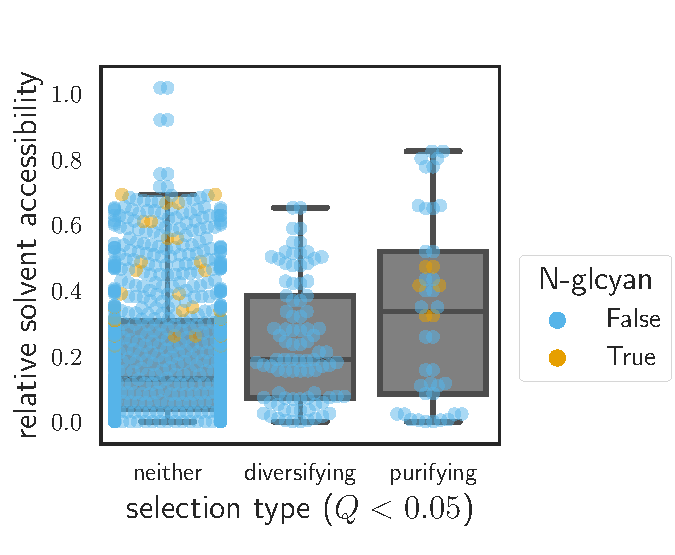
\includegraphics[width=0.5\textwidth]{figures/selsites_rsa.pdf}}
\figsupp[\label{figsupp:slower}Amino-acid preferences and alignment frequencies of sites that evolve slower than expected.]{
This plot shows all sites that are evolving more slowly than expected in natural sequences given the preferences measured in both homologs.
Specifically, it shows all sites with $\omega_r < 1$ at $Q < 0.05$ for the ExpCMs for \emph{both} BG505 and BF520.
For each site, the plots show the preferences averaged across replicates and re-scaled for each homolog, as well as the frequencies of amino acids in the clade A Env alignment. 
The $Q$-value indicated is the maximum of that for the two homologs.
}{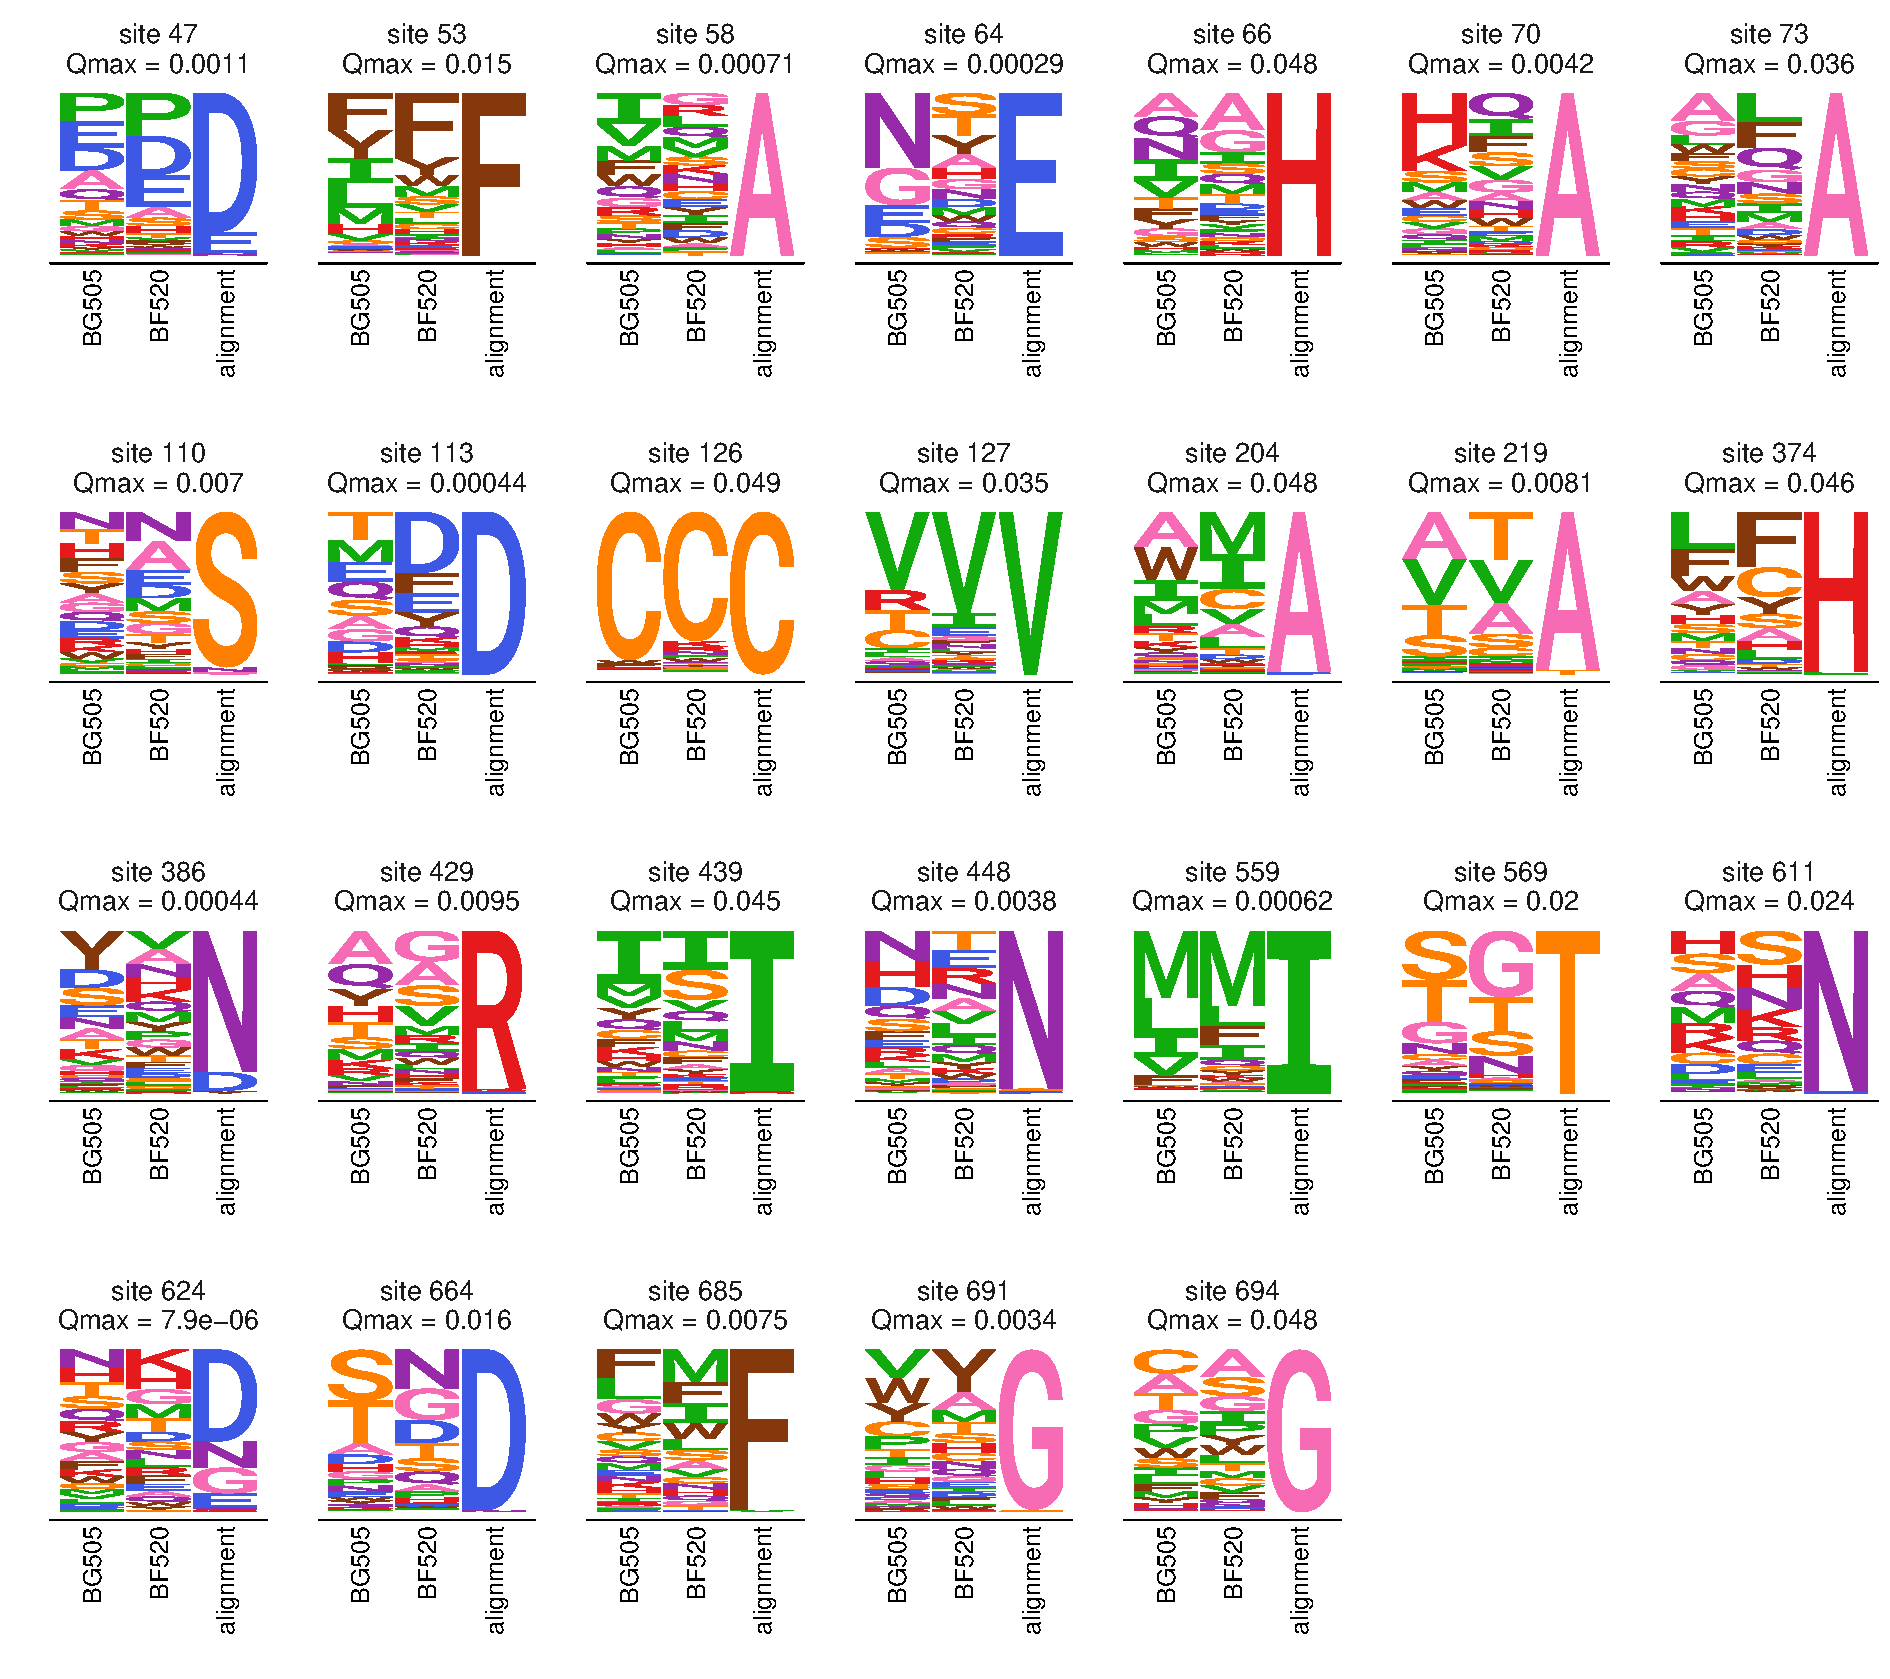
\includegraphics[width=\textwidth]{figures/purifying_selsites.pdf}}
\figdata{The $\omega_r$ and $Q$-values are in \texttt{merged\_omegabysite.csv}.}
\end{figure}

We determined whether each site in Env evolves faster or slower in nature than expected given three models: that evolution is purely neutral (all nonsynonymous and synonymous mutations have equivalent effects), that sites are under the protein-level constraint measured in our experiments with BG505, or that sites are under the constraint measured with BF520. 
The first model used a standard dN/dS test~\citep[the ``FEL'' method of][]{kosakovsky2005not}, whereas the other two models performed a conceptually similar test but used ExpCM that incorporate experimental measurements as described by \citet{bloom2017identification}.
The standard dN/dS model finds hundreds of sites evolve slower than expected under neutral evolution, and only a handful of sites evolve faster than expected under neutral evolution (Table~\ref{tab:phydms}).
This finding is unsurprising, since it is well known that Env is under functional constraint and so has many sites that evolve non-neutrally.
In contrast, ExpCM that test the rates of evolution relative to the experimentally measured constraints find far fewer sites that evolve slower than expected, but many more sites that evolve faster (Table~\ref{tab:phydms}). 

The sites that evolve slower or faster than expected from the experiments are shown in Figure~\ref{fig:divsel}A,B, and also overlaid on the logoplots in Figures~\ref{fig:BG505prefs} and \ref{fig:BF520prefs} as the $\omega_r$ values.
The identified sites are similar regardless of whether we use the experiments with BG505 or BF520 (Figure~\ref{fig:divsel}C).
The reason the results are similar for both experimental datasets is that (as discussed above) the amino-acid preferences of \emph{most} sites are similar in both Envs, meaning that either dataset provides a reasonable approximation of the site-specific functional constraints across the clade A Envs in Figure~\ref{fig:tree}.

What causes some sites to evolve faster or slower in nature than expected from the experiments?
The answer in both cases is likely to be immune selection.
Most of the sites of faster-than-expected evolution are on the surface of Env (Figure~\ref{fig:divsel}A,B and Figure~\ref{fig:divsel}-Figure~supplement~\ref{figsupp:slower}).
Env's escape from autologous neutralizing antibodies often involves amino-acid substitutions in surface-exposed regions~\citep{moore2009specificity}, including at many of the sites that evolve faster than expected.
Since our deep mutational scanning did not impose antibody pressure, sites where substitutions are antibody-driven will evolve faster in nature than expected from the experiments.
Interestingly, immune selection also offers a plausible explanation for the sites that evolve \emph{slower} than expected.
In addition to escaping immunity via substitutions at antibody-binding footprints, Env is notorious for employing a range of more general strategies to reduce its susceptibility to antibodies.
These strategies include shielding immunogenic regions with glycans~\citep{wei2003antibody,stewart2016trimeric} or hiding them by adopting a closed protein conformation~\citep{kwong2002hiv,guttman2015antibody,ozorowski2017open}.
Sites that contribute to such general immune-evasion strategies will be under a constraint in nature that is not present in our experiments -- and indeed, such sites evolve more slowly than expected from our experiments.
For instance, sites of N-linked glycans change slower than our experiments suggest is required by mere functional selection (Figure~\ref{fig:divsel}C), as do sites that help regulate Env's transition between open and closed conformations that have different antibody susceptibilities (Figure~\ref{fig:divsel}D).
Therefore, we can distinguish evolutionary patterns that are shaped by simple selection for Env function from those that are due to the additional complex pressures imposed during human infections. 

\section{Discussion}
We experimentally estimated the effects of all single amino-acid changes to two Env homologs with 85\% amino-acid identity.
We did so using a high-throughput technique called deep mutational scanning.
For each homolog, this approach involved making libraries of \textit{env} with random codon mutations, selecting for mutations that supported viral replication in cell culture, and then deep sequencing the starting and ending libraries to quantify the effect of each mutation.
These experiments imposed strong purifying selection, as indicated by the near-complete depletion of mutations leading to premature stop codons.
For each homolog, the results allowed us to estimate each site's preference for each of the 20 amino acids.
We found that these estimates were largely repeatable between experimental replicates of the same homolog.

We then compared site-specific amino-acid preferences between homologs.
In an initial gene-wide comparison, we simply correlated the preferences between homologs across all sites.
We expected that the differences we observed would be due to a combination of true biological differences and experimental noise.
We quantified experimental noise by correlating the preferences between experimental replicates of the same homolog.
When we then correlated the preferences between replicates from different homologs, we found that the correlation was nearly as high as the correlation between replicates from the same homolog, suggesting that the true preferences of each homolog are fairly well conserved.
As a control, we compared Env's preferences with the preferences from a non-homologous protein -- influenza HA -- among sites that overlap in primary sequence of these proteins.
As expected, the correlation in preferences between these non-homologous proteins was very low.
This finding provided the first indication that although Env's preferences differ to some extent between homologs, they are still much more conserved than expected for two non-homologous proteins.

Next, we quantified shifts in Env's amino-acid preferences at a more site-specific level.
We computed shifts using a metric that takes into account experimental noise.
At each site, this metric estimates the expected shift due to the noise, as captured by experimental replicates, and then corrects for this noise when measuring the shifts between homologs.
We found that for most sites, the shifts between homologs were small-to-intermediate in effect size, with only a few sites having large shifts.
We used the same metric to compare Env and influenza HA at sites that overlap in primary sequence.
As expected for two non-homologous proteins, we found that most sites had large shifts in mutational effects.
Thus, this site-specific analysis provided additional support that the shifts observed between Env homologs were not nearly as large as shifts between non-homologous proteins.

Overall, these results help elucidate the strength of epistasis in Env's long-term evolution.
Although large shifts in mutational effects can occur during protein evolution, our results indicate that such events were rare for the Env homologs we analyzed.
Deep mutational scanning has also been used to analyze mutational shifts between other homologs.
One study compared two homologs of influenza's nucleoprotein with 94\% amino-acid identity~\cite{doud2015site}.
This study found that most mutational effects were conserved.
A lower-throughput study of nucleoprotein mutations with a variety of stability effects found that these effects were also largely conserved among homologs that ranged from 94\%-72\% amino-acid identity~\cite{ashenberg2013mutational}.
Another deep mutational-scanning study compared three homologous TIM-barrel proteins, each with 30-40\% amino-acid identity to one another~\cite{chan2017correlation}.
Even for these considerably divergent homologs, mutational effects were still found to be correlated between homologs at many sites.
Thus, our findings with Env are qualitatively similar to the above studies in suggesting that although epistasis can cause mutational effects to diverge over time, it does not usually completely erase site-specific preferences.

Our results also shed light on the evolutionary basis of shifts in mutational effects.
The deep mutational scan comparing nucleoprotein homologs found that shifts were enriched at sites that differed in wildtype amino-acid sequence between homologs~\cite{doud2015site}.
This trend might be expected if proteins quickly evolve to accommodate historical amino-acid changes, as suggested from computational modeling~\cite{pollock2012amino}.
However, the median shift in Env's preferences was similar between sites that were the same vs. different in wildtype sequence.
Additional comparisons will be required to determine which pattern is more typical.

Future work could expand upon our findings to analyze other Env homologs and the effects of mutations on other Env phenotypes.
In this study, we compared two homologs from subtype A.
It is possible that mutational effects are more shifted between more divergent Envs.
Deep mutational scanning of Env from a different subtype could address this question (our previous results for LAI are difficult to compare with BG505 and BF520, for reasons described above).
The specific phenotype we selected for in our study was the ability of Env to support viral replication in cell culture in the \textit{absence} of immune selection (e.g., antibodies).
However, it is of great interest to characterize the effects of mutations to Env on antibody escape, especially for antibodies being used in immunotherapies or as templates in vaccine design.
We have previously used deep mutational scanning to comprehensively identify single amino-acid mutations that allow BF520 Env to escape a bNAb~\cite{dingens2017comprehensive}.
This technique, when applied to two different Env homologs, could be used to comprehensively determine the extent to which antibody-escape mutations have shifted during Env evolution.


\section{Methods and Materials}

\subsection{Sequence numbering}
We use the HXB2 numbering system \cite{korber1998numbering} for each Env homolog unless otherwise noted.
We defined Env's ``variable loops'' according to \url{http://www.hiv.lanl.gov/}, but did not consider the disulfide-bonded cysteines as part of the loops.

\subsection{Codon-mutant libraries}
For BF520 \textit{env}, we used the codon-mutant libraries generated from a previous study \cite{dingens2017comprehensive}.
For BG505 \textit{env}, we generated codon-mutant libraries using essentially the same methods as the previous study, but with a few modifications.
We computationally generated the sequences of the codon-tiling primers for the PCR-mutagenesis step using the same approach as in~\cite{dingens2017comprehensive}.
The sequences of these primers will be made available as a supplemental file upon publication of this work.
The end primers for this mutagenesis step were: 5'-tgaaggcaaaactactggtccgtctcgagcagaagacagtggcaatgaga-3' and 5'-gctacaaatgcatataacagcgtctcattctttccctaacctcaggcca-3'.
As with BF520, we cloned the BG505 \textit{env} libraries into the \textit{env} locus of the full-length proviral genome of HIV strain Q23 \cite{poss1999variants} -- another subtype-A transmitted/founder virus, using the same high-efficiency cloning vector used previously \cite{dingens2017comprehensive}.
To do so, we first digested the cloning vector with BsmBI.
We then used PCR to elongate the amplicons to include on either end 30 basepairs that are identical in sequence to the ends of the BsmBI-digested vector.
The primers we used for this PCR were:
5'-agataggttaattgagagaataagagaaagagcagaagacagtggcaatgagagtgatgg-3' and 5'-ctcctggtgctgctggaggggcacgtctcattctttccctaacctcaggccatcc-3'.
Next, we used NEBuilder HiFi DNA Assembly (NEB, E2621S) to clone the \textit{env} amplicons into the BsmBI-digested plasmids.
We purified the assembled products using Agencourt AMPure XP beads (Beckman Coulter, A63880) using a bead-to-sample ratio of 1.5, and then transformed the purified products into Stellar electrocompetent cells (Takara, 636765).
The transformations yielded between 1.5-3.6 million unique clones for each of the three replicate libraries, as estimated by plating 1:2,000 dilutions of the transformations.
As before, we scraped the plated colonies and maxiprepped the plasmid DNA, but this time we did not include the 4-hour outgrowth step after the scraping step.
For the wildtype controls, we maxiprepped three independent cultures of wildtype BG505 \textit{env} in the \textit{env} locus of the full-length Q23 proviral plasmid.

\subsection{Generation and passaging of viruses}
For BF520, we analyzed the viruses generated and passaged in our previous study \cite{dingens2017comprehensive}.
For BG505, we generated and passaged viral libraries using essentially the same methods.
First, for each replicate, we generated mutant viruses by transfecting 293T cells in three 6-well plates with a mixture of 2 ug mutant plasmid DNA and 6 uL FuGENE 6 Transfection Reagent (Promega, E269A) and 100 uL DMEM per well.
293T cells were seeded in D10 media (DMEM supplemented with 10\% FBS, 1\% 200 mM L-glutamine, and 1\% of a solution of 10,000 units/mL penicillin and 10,000 $\mu$g/mL streptomycin) the day before transfection with 0.5 million cells per well, such that they were approximately 50\% confluent the next day.
In parallel, we generated wildtype viruses by transfecting one 6-well plate of 293T cells with wildtype plasmid, using the same amount of DNA and transfection reagent as above.
At 2days post-transfection, we harvested the transfection supernatant, passed it through a 0.2$\mu$m filter, treated the supernatant with DNAse to digest residual plasmid DNA (as in~\cite{haddox2016experimental}), and froze aliquots at -80$^{\circ}$C.
We thawed and titered aliquots using the TZM-bl assay in the presence of 10 $\mu$g/mL DEAE-dextran as described in~\cite{dingens2017comprehensive}.

Next, we conducted the initial viral passage in SupT1.CCR5 cells (obtained from Dr. James Hoxie \cite{boyd2015mutations}).
During this passage, cells were maintained in R10 media, which has the same composition as D10 (described above), but has RPMI-1640 (GE Healthcare Life Sciences, SH30255.01) in the place of DMEM, with 10 $\mu$g/mL DEAE-dextran to enhance viral infection.
We infected cells with 4 million (for replicate 1) or 5 million (for replicates 2 and 3) TZM-bl infectious units of mutant virus at an MOI of 0.01, with cells at a starting concentration of 1 million cells/mL in vented tissue-culture flasks (Fisher Scientific, 14-826-80).
At 1 day post-infection, we pelleted cells, aspirated the supernatant, and resuspended cell pellets in fresh media including DEAE-dextran.
At 2 days post-infection, we doubled the volume of each culture with fresh media including DEAE-dextran.
At 4 days post-infection, we pelleted cells, passed the virus-containing supernatant through a 0.2 $\mu$m filter, concentrated the virus $\sim$30 fold using ultracentrifugation as described in~\cite{dingens2017comprehensive}, and then froze aliquots at -80$^{\circ}$C.
In parallel, for each replicate, we also passaged 0.2 million (for replicate 1) or 0.5 million (for replicates 2 and 3) infectious units of wildtype virus with and using the same conditions.
We thawed and titered these aliquots using the TZM-bl assay in the presence of 10 $\mu$g/mL DEAE-dextran.

We conducted a second, much shorter viral passage by infecting cells with the passage-1 viruses.
For each virus, we infected 1 million TMZ-bl infectious units into 1 million SupT1.CCR5 cells in the presence of 100 $\mu$g/mL DEAE-dextran (a 10-fold higher concentration than to concentration we used in the TZM-bl assay to titer the virus, meaning the actual number of infectious units in this passage was probably higher).
Three hours post-infection, we pelleted the cells and resuspended them in fresh media without any DEAE-dextran.
At 12 hours post-infection, we pelleted cells, washed them once with PBS, and then used a miniprep kit to harvest reverse-transcribed unintegrated viral DNA.

\subsection{Generation of samples for Illumina sequencing}
We deeply sequenced each plasmid library before selection and each viral library after the two passages, as well as the wildtype plasmids and wildtype viruses that served as controls.
First, we generated PCR amplicons of \textit{env} using the same approach as~\cite{dingens2017comprehensive} with the primers: 5'-GAAGACAGTGGCAATGAGAGTGATGG-3' and 5'-TTCCCTAACCTCAGGCCATCC-3'.
Next, we sequenced these amplicons using a barcoded sub-amplicon sequencing strategy to reduce the sequencing error rate, as previously described~\cite{doud2016accurate,haddox2016experimental}, dividing \textit{env} into seven amplicons.
The primer pairs used to generate these subamplicons are as follows, where N characters represent randomized sites in the barcode region of the primer:

\begin{itemize}
{\footnotesize
\item 5'-CTTTCCCTACACGACGCTCTTCCGATCTNNNNNNNNGATCTTGGGGATGATAATAATCTGTAGTGC-3' and 5'-GGAGTTCAGACGTGTGCTCTTCCGATCTNNNNNNNNGGTGACATTGGTACACTGTAGAGTAAC-3'
\item 5'-CTTTCCCTACACGACGCTCTTCCGATCTNNNNNNNNCCATGTGTAAAGTTAACCCCTCTCTGC-3' and 5'-GGAGTTCAGACGTGTGCTCTTCCGATCTNNNNNNNNGAACTTCTTATCCTTACACTTTAGGATCGC-3'
\item 5'-CTTTCCCTACACGACGCTCTTCCGATCTNNNNNNNNCATACATTATTGTGCCCCAGCTGG-3' and 5'-GGAGTTCAGACGTGTGCTCTTCCGATCTNNNNNNNNCAATGTGCTTGTCTTATATCCCCTATTATGTC-3'
\item 5'-CTTTCCCTACACGACGCTCTTCCGATCTNNNNNNNNGGACAAGCATTCTATGCAACAGGG-3' and 5'-GGAGTTCAGACGTGTGCTCTTCCGATCTNNNNNNNNTGCTTTATTCTGCATGGGAGAGTTATAC-3'
\item 5'-CTTTCCCTACACGACGCTCTTCCGATCTNNNNNNNNGTCAAATAGCACGGGGTCAAATGAC-3' and 5'-GGAGTTCAGACGTGTGCTCTTCCGATCTNNNNNNNNCCAAGGAAGACAGCTCCTATTCCAAC-3'
\item 5'-CTTTCCCTACACGACGCTCTTCCGATCTNNNNNNNNGTGGTGGGGAGAGAAAAAAGAGC-3' and 5'-GGAGTTCAGACGTGTGCTCTTCCGATCTNNNNNNNNGTTTCTATTACTCCAACTAGAGTTCCAGGG-3'
\item 5'-CTTTCCCTACACGACGCTCTTCCGATCTNNNNNNNNGGAAAACTCATCTGCACCACTAATGTG-3' and 5'-GGAGTTCAGACGTGTGCTCTTCCGATCTNNNNNNNNTGAGTATCCCTGCCTAACTCTATGTATTACAG-3'
}
\end{itemize}

The resulting deep-sequencing data will be made available on the Sequence Read Archive upon the publication of this work.

\subsection{Analysis of deep-sequencing data}

We analyzed the deep-sequencing data using the \texttt{dms\_tools} software package~\cite{bloom2015software}.
The specific code we used will be made available upon the publication of this work.
A summary of our workflow is as follows, and involves multiple programs encoded in \texttt{dms\_tools}:
First, we aligned sequencing reads to \textit{env} and computed site-specific codon mutation frequencies using \texttt{dms\_barcodedsubamplicons}, using \texttt{dms\_summarizealignments} to make plots summarizing these frequencies.
Next, we inferred Env's preferences from the codon counts using \texttt{dms\_inferprefs}.
We then used a custom script to compare these preferences between homologs.

\subsection{Alignments and phylogenetic analyses of HIV-1 {\it env} sequences}
We made the trees in Fig \ref{ref:ch3_tree} using multiple-sequence alignments downloaded from the HIV sequence database (\url{http://www.hiv.lanl.gov/}) that we then manually curated in the following ways:
First, we removed sequences that differed in length from the HXB2 reference sequence (including gap characters), or which contained a premature stop codon, ambiguous residue, or frame-shift mutation.
Next, we removed columns in the alignment for which we lack deep mutational scanning data or are not present in HXB2, columns that have $>$5\% gap characters, or columns in variable loops that looked poorly aligned by eye.
The sequences used to make the trees in Fig \ref{ref:ch3_tree} were randomly selected from the larger alignment, with a defined number of sequences per clade, as described in the figure.
The topologies of these trees were inferred by \texttt{RAxML} using the GTRCAT model.
In the \texttt{phydms}~\cite{hilton2017phydms} analyses, we fixed the topologies of these trees, and then compared the ability of the different models to optimize the branch lengths.
The trees shown in Fig \ref{ref:ch3_tree} are the results of optimizing the branch lengths using the YNGKP M5 model.
The code we used to generate these alignments, build the trees, and conduct the \texttt{phydms} analyses will be made available upon publication of this work.

\subsection{Preference differences}Next, we sought to quantify shifts in Env's preferences at a site-specific level.
Correlating preferences between replicates of the same homolog showed that some sites were substantially influenced by experimental noise Fig \ref{fig:ch3_homologs_corr}.
Thus, we quantified shifts using an approach that corrects for noise, similar to the one used in a previous study that deep mutational-scanning data between homologs of influenza's nucleoprotein \cite{doud2015site}.
Fig \ref{fig:ch3_distances}A shows how we quantified shifts for a few example sites.
For a given site $r$, we define the distance in preferences between an arbitrary pair of replicates $i$ and $j$ as: $D_{r}^{i,j} = \frac{1}{2}\sum_{a}|\pi_{r,a}^{i}-\pi_{r,a}^{j}|$.
We then use this metric to measure the distance between all pairwise combinations of replicates from both homologs.
We quantified the un-corrected distance between homologs as the root mean square of all replicate-replicate distances between homologs ($RMSD_{between}$).
Since $D_{r}^{i,j}$ can range between 0-1, $RMSD_{between}$ also ranges between 0-1, with 0 indicating no differences and 1 indicating extreme differences between the homologs.
Next, we quantified experimental noise as the root mean square of all replicate-replicate distances where both replicates came from the \textit{same} homolog ($RMSD_{within}$).
Finally, we computed the noise-corrected distance between homologs ($RMSD_{corrected}$) by subtracting $RMSD_{between}$ by $RMSD_{within}$.

Sites where we repeatedly measured large differences between homologs are expected to have $RMSD_{corrected}$ values much greater than zero (e.g., sites 512 and 309; Fig \ref{fig:ch3_distances}A).
In contrast, sites where we repeatedly measured small differences between homologs are expected to have $RMSD_{corrected}$ values close to zero (e.g., site 296).
Sites where the noise completely overwhelmed the biological signal are also expected to have $RMSD_{corrected}$ values close to zero (e.g., site 607).
Thus, a $RMSD_{corrected}$ value near zero could indicate that a site's preferences are conserved between homologs, or that the noise at a site is high.



\section{Acknowledgments}
We thank Michael Doud and Orr Ashenberg for computer code that formed the basis for some of the analyses.
We thank Andrew Ward for pointing out to us that some of the sites with slower-than-expected rates of evolution are involved in Env's conformational changes upon receptor binding.
We thank Kelly Lee for helpful input about the relative stabilities of the BG505 and BF520 Envs.
\jdbcomment{add more}

\bibliography{references.bib}

\clearpage

\begin{suppfile}
\caption{
\label{suppfile:code}
The code to perform all steps in the analysis is in \texttt{analysis\_code.zip}.
Specifically, this file contains a Jupyter notebook that performs the analysis, all required input data, and all reasonably sized output files.
The Jupyter notebook downloads the deep sequencing data, processes it with the \texttt{dms\_tools2} software~\citep[\url{https://jbloomlab.github.io/dms_tools2/}]{bloom2015software}, and also performs a variety of downstream analyses that generate most of the figures for this paper.
}
\end{suppfile}

\begin{suppfile}
\caption{
\label{suppfile:html}
An HTML rendering of the Jupyter notebook that performs the computational analysis.
The actual notebook is in Supplementary~file~\ref{suppfile:code}, but if you just want to look at the analysis rather than run it, then you may prefer this file instead.
In particular, the notebook contains plots detailing the deep sequencing data analysis as generated using the \texttt{dms\_tools2} software~\citep[\url{https://jbloomlab.github.io/dms_tools2/}]{bloom2015software}.
}
\end{suppfile}


\end{document}
